\section{Experimental evaluation}\label{sec:exper}
We conducted an experimental evaluation of our algorithms, with two major
driving goals in mind: to study the behavior of the algorithms presented in this
paper and to compare it with that of other related
algorithms~\citep{Brandes01,BrandesP07,JacobKLPT05,GeisbergerSS08}, in terms of
accuracy of the estimation, execution time, work performed, and scalability as
function of the network size. 

\paragraph{Implementation and environment}
We implemented\footnote{We plan to make our software available after
acceptance.} our algorithms, the one presented in~\citep{BrandesP07,JacobKLPT05}
and the linear scaling version from~\citep{GeisbergerSS08} in C, by extending
the implementation of the exact algorithm~\citep{Brandes01} contained in
igraph~\citep{igraph}. The implementations are similarly engineered, given that
they are based on the same subroutines for the computation of the shortest path
(Dijkstra's algorithm for weighted graphs, BFS for unweighted ones), and they
received similar amounts of optimization. We exposed our implementations through
Python 3.3.1, which was used for running the simulations. We run the experiments
on a quad-core AMD Phenom\texttrademark II X4 955 Processor with 16GB of RAM,
running Debian \emph{wheezy} with a Linux kernel version 3.2.0.

\paragraph{Datasets} We used a number of graphs from the Stanford Large
Network Dataset
Collection\footnote{\url{http://snap.stanford.edu/data/index.html}}. These are
all real world datasets including online social networks, communication (email)
networks, scientific citation and academic collaboration networks, road
networks, Amazon frequent co-purchased product networks, and more. Basic
information about the graphs we used are reported in the leftmost part
of~\cref{tab:expDir,tab:expUndir} \XXX May I suggest we use package
ctable for the tables? They look much better. We refer the
reader to the SLNDC website for additional details about each dataset. 
To evaluate scalability we also created a number of artificial graphs of
different sizes (1,000 to 100,000 vertices) using the Barab\'asi-Albert
model~\citep{BarabasiA99} as implemented by igraph~\citep{igraph}. \XXX Are
there parameters of the Barabasi-Albert model we should mention?

\paragraph{Diameter approximation}
As we discussed in the previous sections the number of samples that the proposed
algorithm requires depends on the vertex-diameter of the graph. 
For the computation of the vertex-diameter in case of undirected graphs we used
the 2-approximation algorithm that we briefly described in Sect.~\ref{sec:algo}.
We denote this as ``diam-2-approx'' when reporting results in this section. For
directed graphs, we computed the number of samples using both the exact value of
the vertex-diameter (indicated as diam-exact) as well as the trivial upper bound
$|V|-1$ (indicated as diam-UB). 

\XXX In the rest of the section we never say which of our algorithms we are
evaluating. We should be more explicit, especially if we include results for
multiple algorithms/variants.

\begin{table*}[ht]
%\caption{Experiments on Undirected Graphs} % title of Table
\centering % used for centering table
  \begin{small}
\begin{tabular}{|c c c c |c c |c  c |} % centered columns (5 columns)
\hline\hline %inserts double horizontal lines
Graph & Node & Edges & Diameter  & \multicolumn{2}{|c|}{$\frac{\varepsilon\mbox{-Edges-BP}}{ \varepsilon\mbox{-Edges-VC}}$} & \multicolumn{2}{c|}{$\frac{\varepsilon\mbox{-Time-BP}}{\varepsilon\mbox{-Time-VC}}$}\\ [0.5ex] % inserts table 
\hline
&  &  & &\multicolumn{4}{|c|}{diam-2-approx} \\
\hline
&  &  & & min & max & min & max\\
%heading
\hline % inserts single horizontal line
%\multirow{6}{35mm}{\begin{sideways}\parbox{15mm}{Undirected\\ diam-approx}\end{sideways}}\\
oregon1-010331 & 10,670 & 22,002 & 9 & 3.69 & 3.73 & 4.39 & 4.75\\  % [1ex] adds vertical space
oregon1-010526 & 11,174 & 23,409 & 10 &  3.53 & 3.74 & 4.26 & 4.73 \\
ca-HepPh & 12,008 & 237,010 & 13  & 2.43 & 2.49 & 3.06 & 3.33\\
ca-AstroPh & 18,772 & 396,160  & 14  & 2.81 & 2.95 & 3.26 & 3.76\\
ca-CondMat & 23,133 & 186,936 & 15  & 3.24 & 3.26 & 3.75 & 4.08\\
email-Enron & 36,692 & 421,578 & 12  & 2.98 & 3.18 & 3.60 & 4.16\\[1ex] % inserting body of the table
\hline %inserts single line
\end{tabular}
\end{small}
\caption{\XXX
%For each graph efficiency measures generated  for a given input  as the average of 5 runs for a  pair of given values $\varepsilon,\delta$.
%The value of $\delta$ was 0.1 and $\varepsilon$ took values 0.01, 0.015, 0.02, 0.04, 0.06, 0.08, 0.1.
%Among the 6 data points that produced with varied $\varepsilon$ we present the minimum and maximum ratios of the Brandeis-Pitch method over VC-dimension method for the number of touched edges during the execution and time.
%In both undirected and directed graphs the exact value of the diameter was used. For each ($\varepsilon,\delta$) the experiment was repeated 5 times and the average was recorded.
}
\label{tab:expUndir} % is used to refer this table in the text
\end{table*}

\begin{table*}[ht]
%\caption{Experiments on Directed Graphs} % title of Table
\centering % used for centering table
\begin{small}
\begin{tabular}{|c c c c | c c | c c | c c | c c | c c | c c|} % centered columns (5 columns)
\hline\hline %inserts double horizontal lines
Graph & Node & Edges & Diameter  & \multicolumn{2}{|c|}{$\frac{\varepsilon\mbox{-Edges-BP}}{ \varepsilon\mbox{-Edges-VC}}$} & \multicolumn{2}{c|}{$\frac{\varepsilon\mbox{-Time-BP}}{\varepsilon\mbox{-Time-VC}}$} & \multicolumn{2}{c|}{$\frac{\varepsilon\mbox{-Edges-BP}}{ \varepsilon\mbox{-Edges-VC}}$} & \multicolumn{2}{c|}{$\frac{\varepsilon\mbox{-Time-BP}}{\varepsilon\mbox{-Time-VC}}$} & \multicolumn{2}{c|}{$\frac{\varepsilon\mbox{-Edges-BP}}{ \varepsilon\mbox{-Edges-VC}}$} & \multicolumn{2}{c|}{$\frac{\varepsilon\mbox{-Time-BP}}{\varepsilon\mbox{-Time-VC}}$}\\ [0.5ex] % inserts table 
\hline
&  &  & &\multicolumn{4}{|c|}{diam-exact}  &  \multicolumn{4}{c|}{diam-UB} & \multicolumn{4}{c|}{Top-K}\\
%heading
\hline % inserts single horizontal line
&  &  & &min & max & min & max&min & max & min & max &min & max & min & max\\
\hline % inserts single horizontal line
%\multirow{6}{13mm}{\begin{sideways}\parbox{15mm}{Directed}\end{sideways}}\\
wiki-Vote & 7,115 & 103,689  & 7 & 2.99 & 3.10 & 3.35 & 3.69 & 1.04 & 1.06 &1.05 & 1.27 & - & - & - & -\\
p2p-Gnutella25 & 22,687 & 54,705 & 11 & 5.02 & 5.46 & 5.45 & 5.78 & 1.85& 1.94& 1.94 & 2.09 & - & - & - &-\\
cit-HepTh & 27,770 & 352,807 & 14  & 2.71 & 2.86 & 3.58 & 3.83 & 1.17 & 1.21 & 1.39 & 1.61 & - & -  & - & -\\
cit-HepPh & 34,546 & 421,578 & 12 & 3.51 & 3.68 & 4.91 & 5.01 & 1.20 & 1.25& 1.60 & 1.71 & - & -  &-  &-\\ % inserting body of the table
p2p-Gnutella30 & 36,682 & 88,328 & 10  & 5.33 & 5.63 & 5.02 & 5.46 & 1.92 & 1.99 & 2.08 & 2.22 & - & - & - & -\\
soc-Epinions1 & 75,879 & 508,837 & 13  & 3.06&  3.11 & 4.20 & 4.25 & 1.00 & 1.03 & 1.35 & 1.38 & - &  - & - & -\\ [1ex] % [1ex] adds vertical space
\hline %inserts single line
\end{tabular}
\end{small}
\caption{\XXX
%For each graph efficiency measures generated  for a given input  as the average of 5 runs for a  pair of given values $\varepsilon,\delta$.
%The value of $\delta$ was 0.1 and $\varepsilon$ took values 0.01, 0.015, 0.02, 0.04, 0.06, 0.08, 0.1.
%Among the 6 data points that produced with varied $\varepsilon$ we present the minimum and maximum ratios of the Brandeis-Pitch method over VC-dimension method for the number of touched edges during the execution and time.
%In both undirected and directed graphs the exact value of the diameter was used. For each ($\varepsilon,\delta$) the experiment was repeated 5 times and the average was recorded.
}
\label{tab:expDir} % is used to refer this table in the text
\end{table*}
\subsection{Accuracy}\label{sec:accuracy}
Our theoretical results from Sect.~\ref{sec:algo} guarantee that, with probability
at least $1-\delta$, all estimations of the betweenness values for all vertices
in the graph are within $\varepsilon$ for their real value, that is
\[
\Pr(\exists v\in V \mbox{ s.t. }
|\betw(v)-\tilde\betw(v)|>\varepsilon)<\delta\enspace.
\]
We run our algorithm five times for each graph and each value of $\varepsilon$
in $\{0.01, 0.015, 0.02, 0.04, 0.06, 0.08, 0.1\}$. The parameter $\delta$ was
fixed to $0.1$ and we used $c=0.5$ in~\eqref{eq:vceapprox} to compute the sample
size, as suggested by~\citet{LofflerP09}. As far as the \emph{confidence} is
concerned, we report that in all the hundreds of runs we performed, the
guarantee on the deviation was \emph{always} satisfied, not just with
probability $1-\delta$ (0.9). We evaluated how good the estimated values are is
by computing the average \emph{estimation error} $(\sum_{v\in
V}|\betw(v)-\tilde\betw(v)|)/|V|$ across five runs of our algorithm and taking
the average and the standard deviation of this measure, for different values of
$\varepsilon$. We also compute the maximum error overall. The results are
reported in~\cref{fig:gnutella:error} for the directed graph p2p-Gnutella30, and
in~\cref{fig:email:error} for the undirected graph email-Enron. It is evident
that the maximum error is an error of magnitude smaller than the guaranteed
value of $\varepsilon$ and that the average error is almost two orders of
magnitude smaller than the guarantees, and the average+standard deviation points
show that the estimation are quite concentrated around the average. We can
conclude that in practice the algorithm performs even better than guaranteed,
achieving higher accuracy and confidence than what the theoretical analysis
indicates. This may be due to a number of factors, including the fact that the
vertex-diameter is an \emph{upper bound} to the VC-dimension of the rangeset and
the inherent looseness of the bound to the sample size~\eqref{eq:vceapprox}.

\XXX IS THERE SOMETHING WRONG WITH THIS FIGURES? IT SEEMS STRANGE TO ME THAT IN
FIG 4, THE ESTIMATION USING THE EXACT DIAMETER IS BETTER THAN WITH THE UPPER
BOUND.

\begin{figure*}[ht]
  \centering
  \hfill
  \subfloat[p2p-Gnutella30 (directed)]{\label{fig:gnutella:error}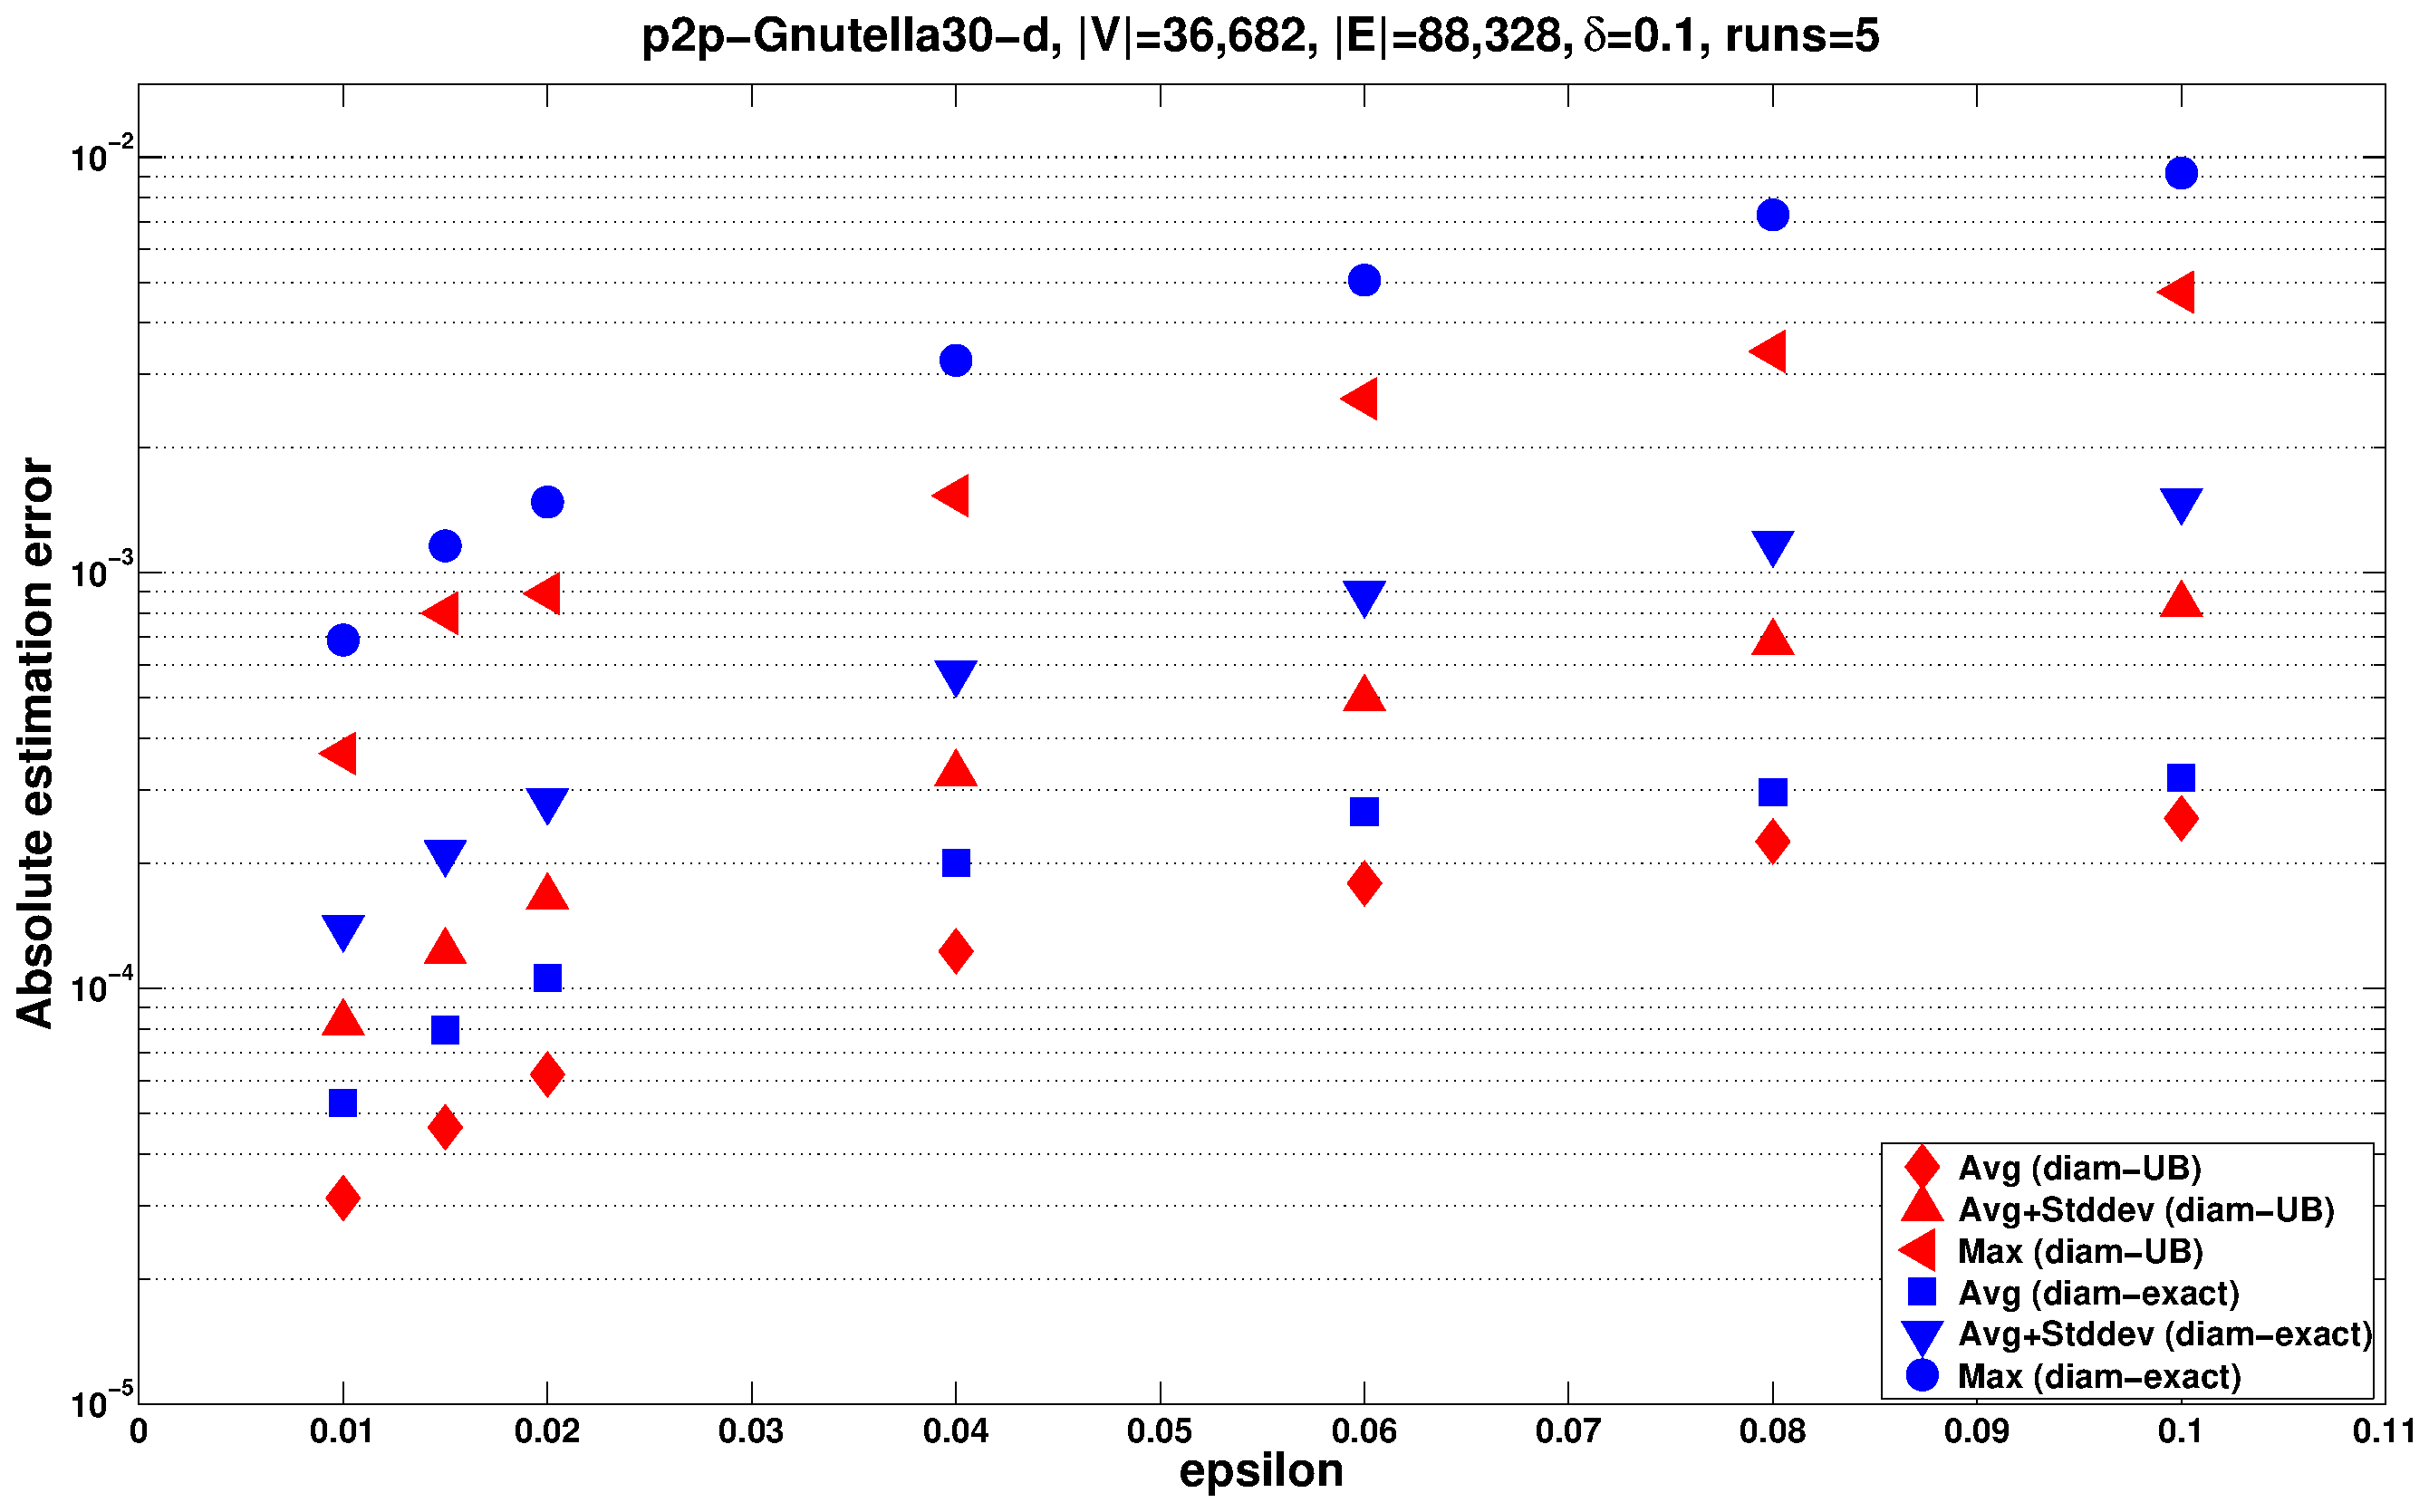
\includegraphics[width=0.45\textwidth,keepaspectratio]{p2p-Gnutella30-error}}
  \hfill
  \subfloat[email-Enron (undirected)]{\label{fig:email:error}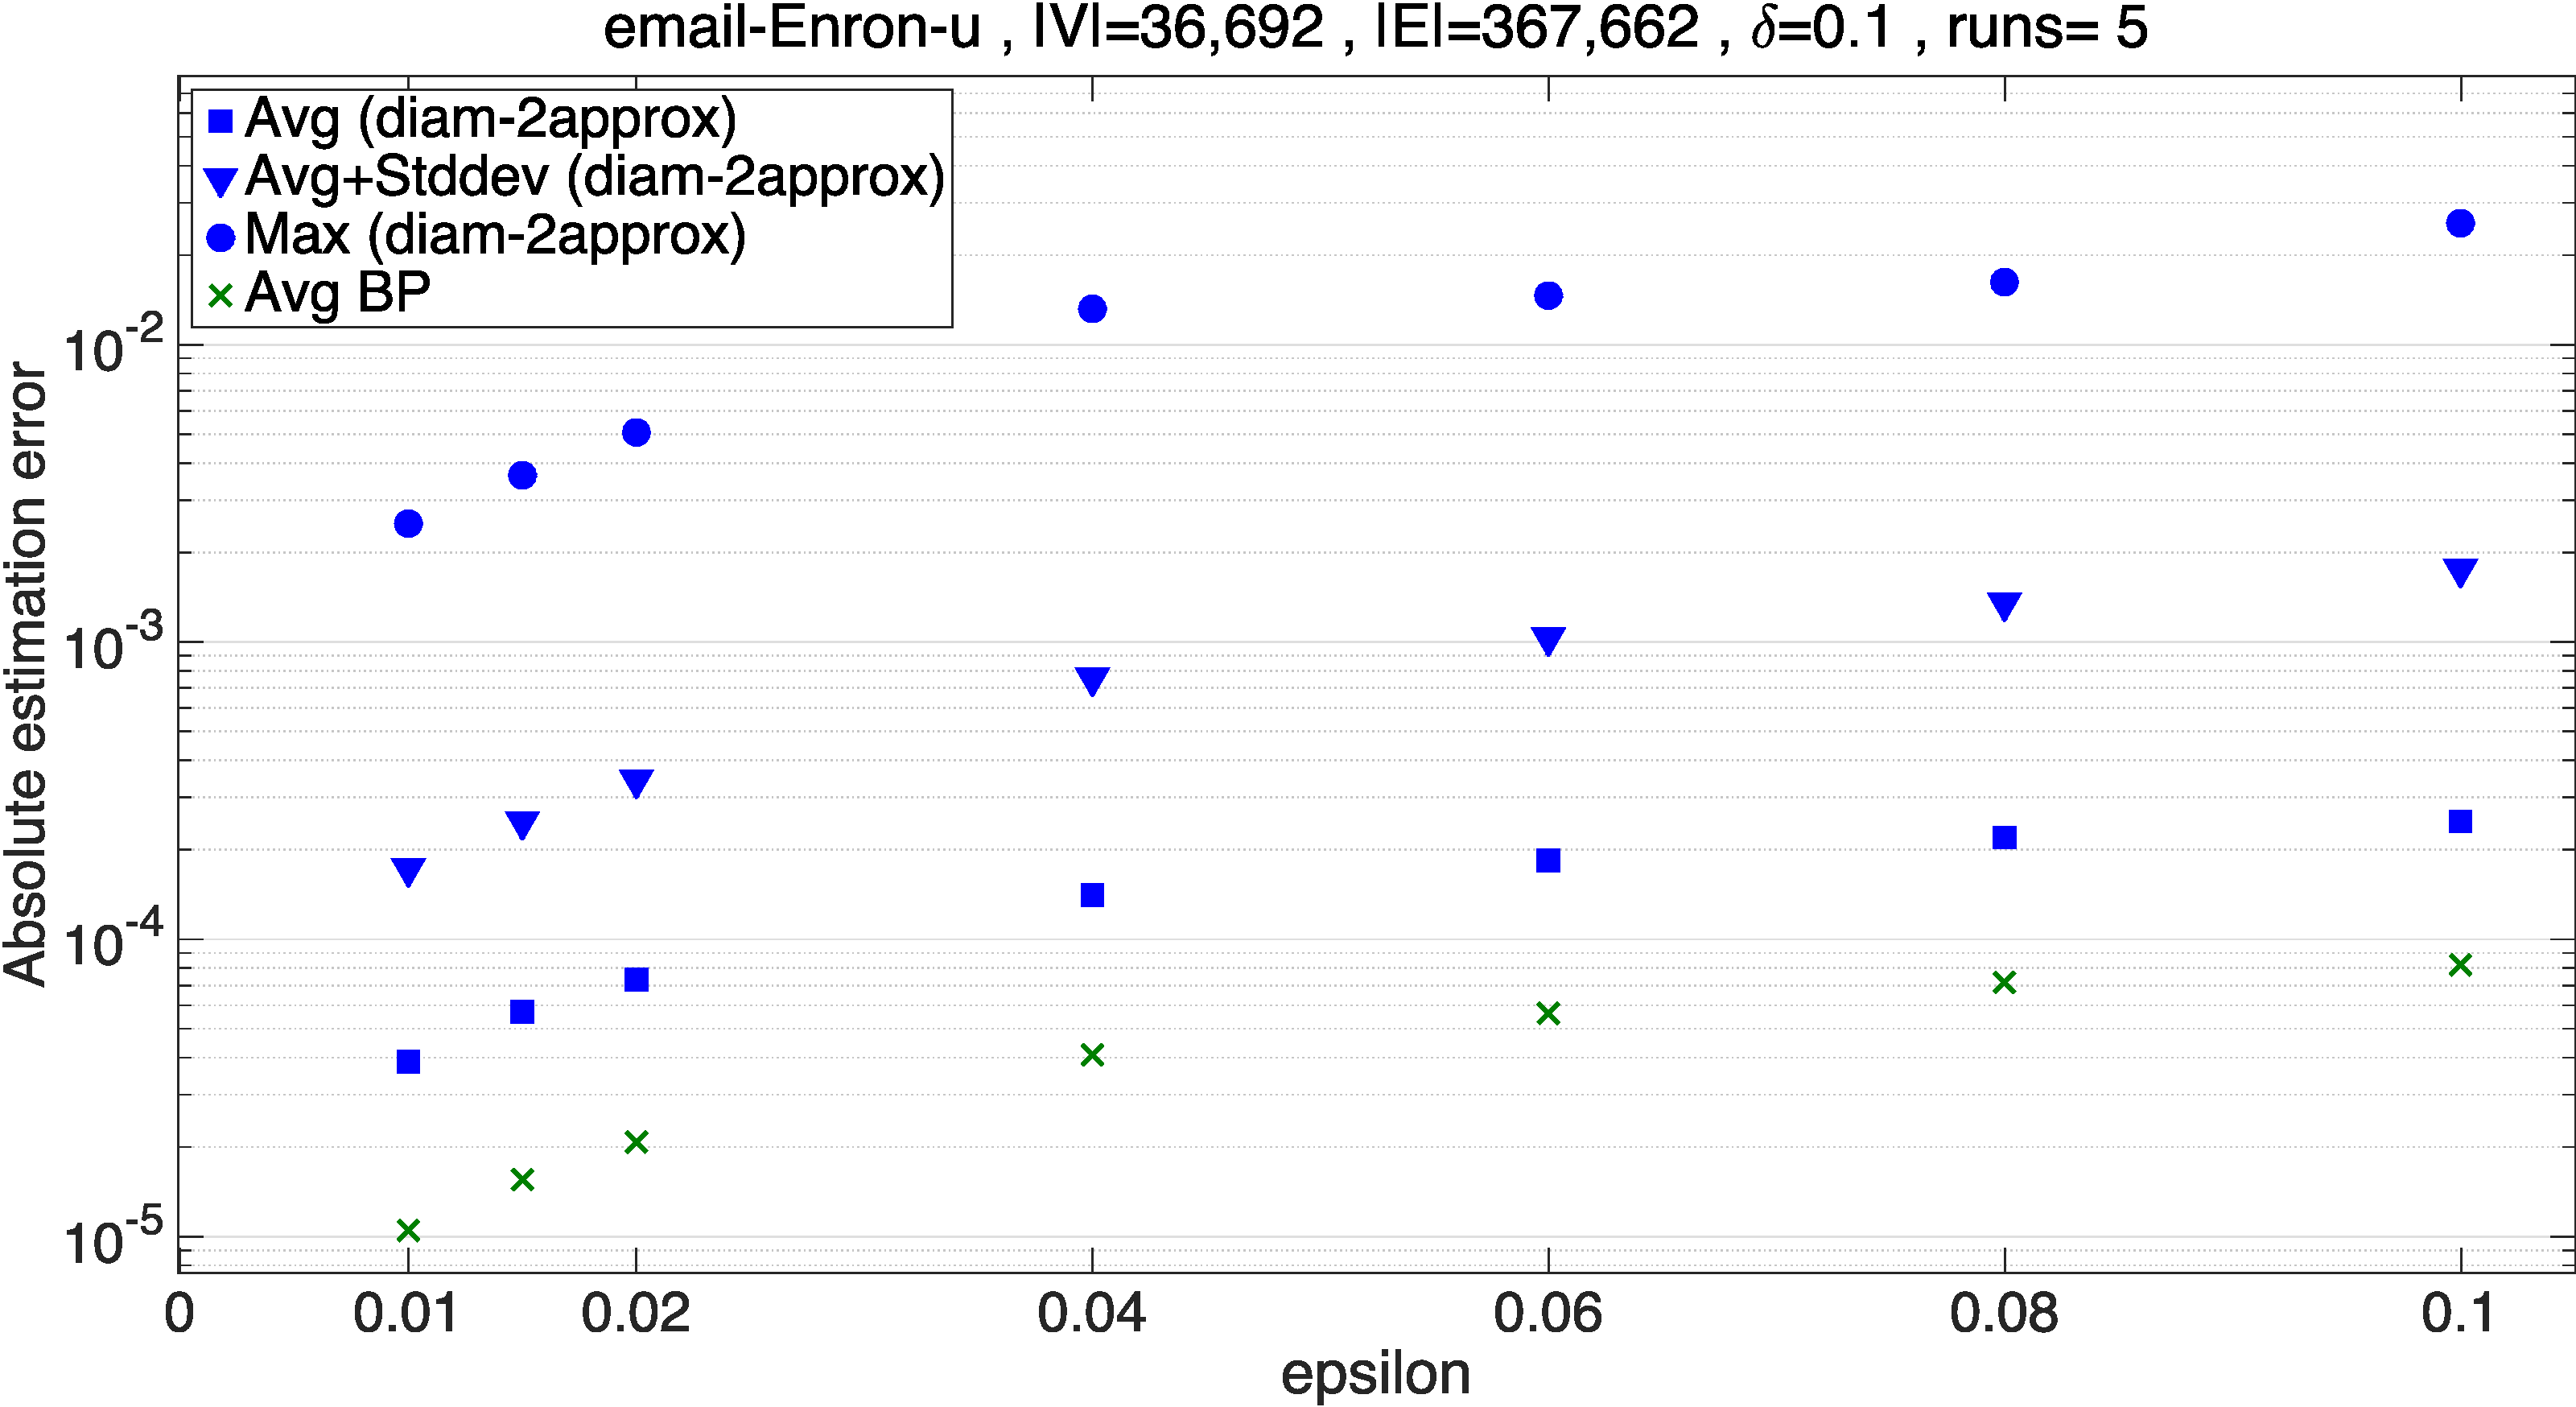
\includegraphics[width=0.45\textwidth,keepaspectratio]{email-Enron-error}}
  \hfill
  \caption{Betweenness estimation error $|\tilde\betw(v)-\betw(v)|$ evaluation
  for directed and undirected graphs} 
  \label{fig:error}
%\begin{minipage}[b]{0.5\linewidth}
%\flushleft
%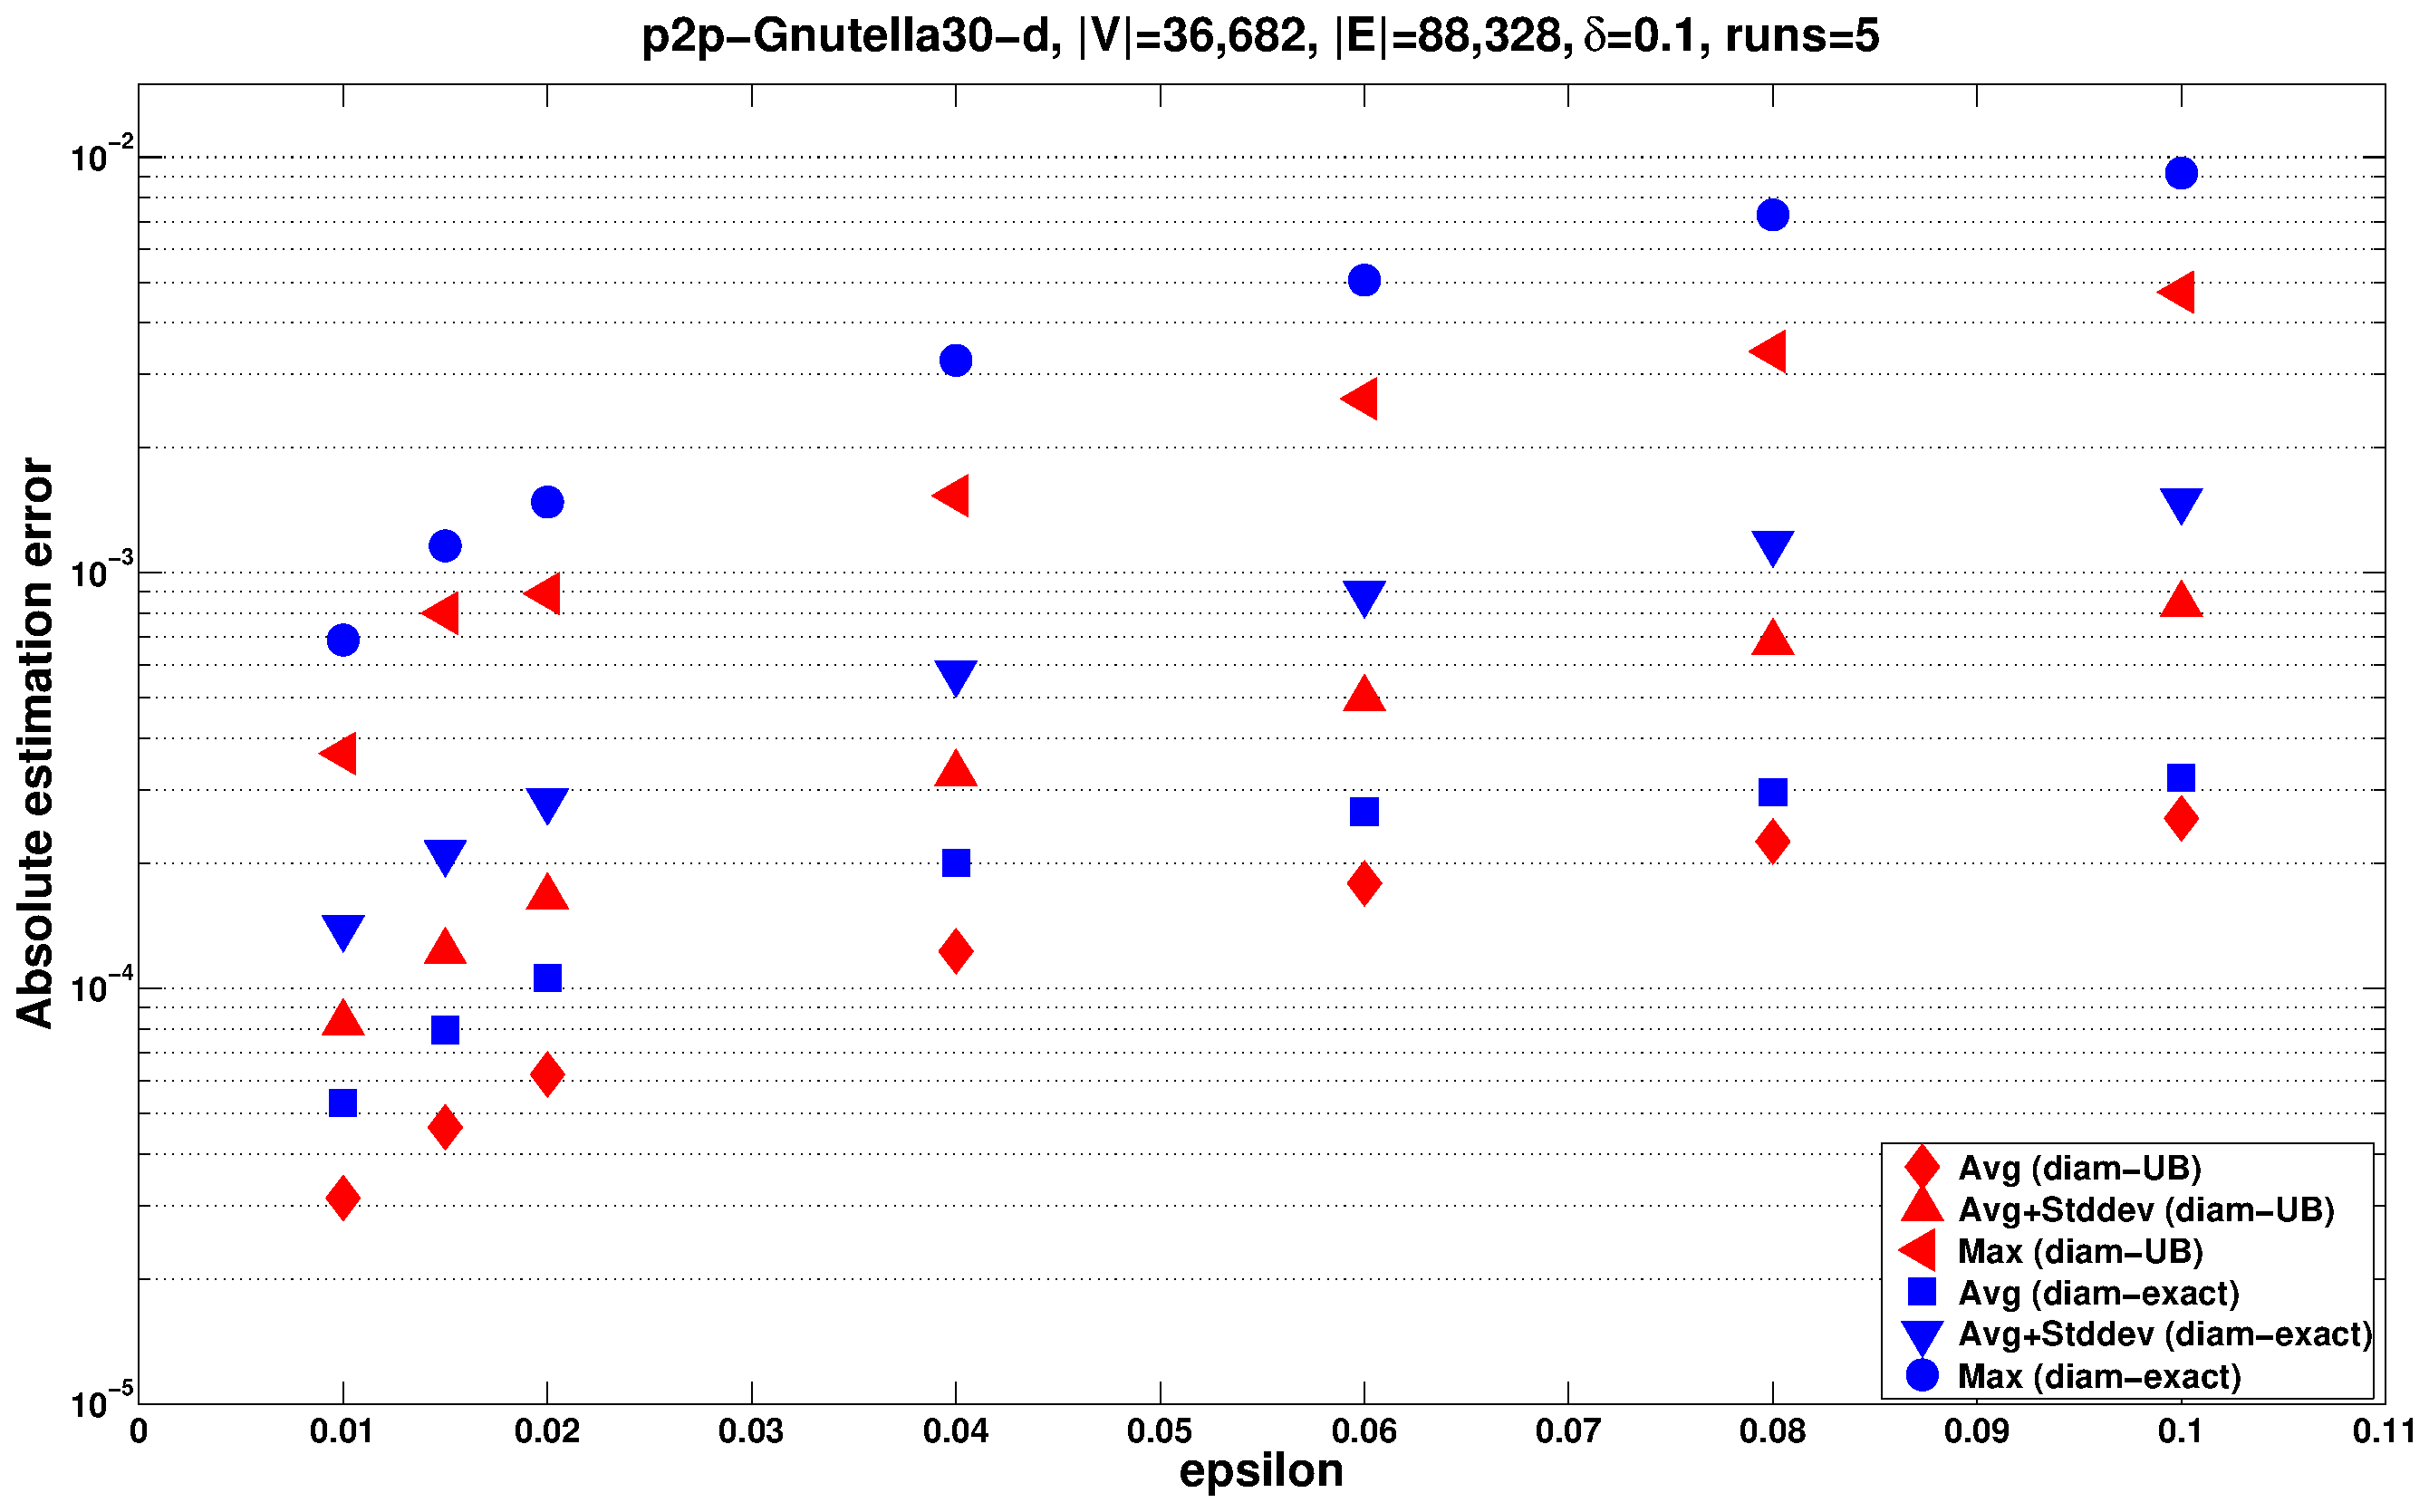
\includegraphics[width=3.8in, keepaspectratio]{p2p-Gnutella30-error.eps}
%\caption{Error evaluation on p2p-Gnutella30} \label{fig:gnutella:error}
%\end{minipage}%
%\begin{minipage}[b]{0.5\linewidth}
%\centering
%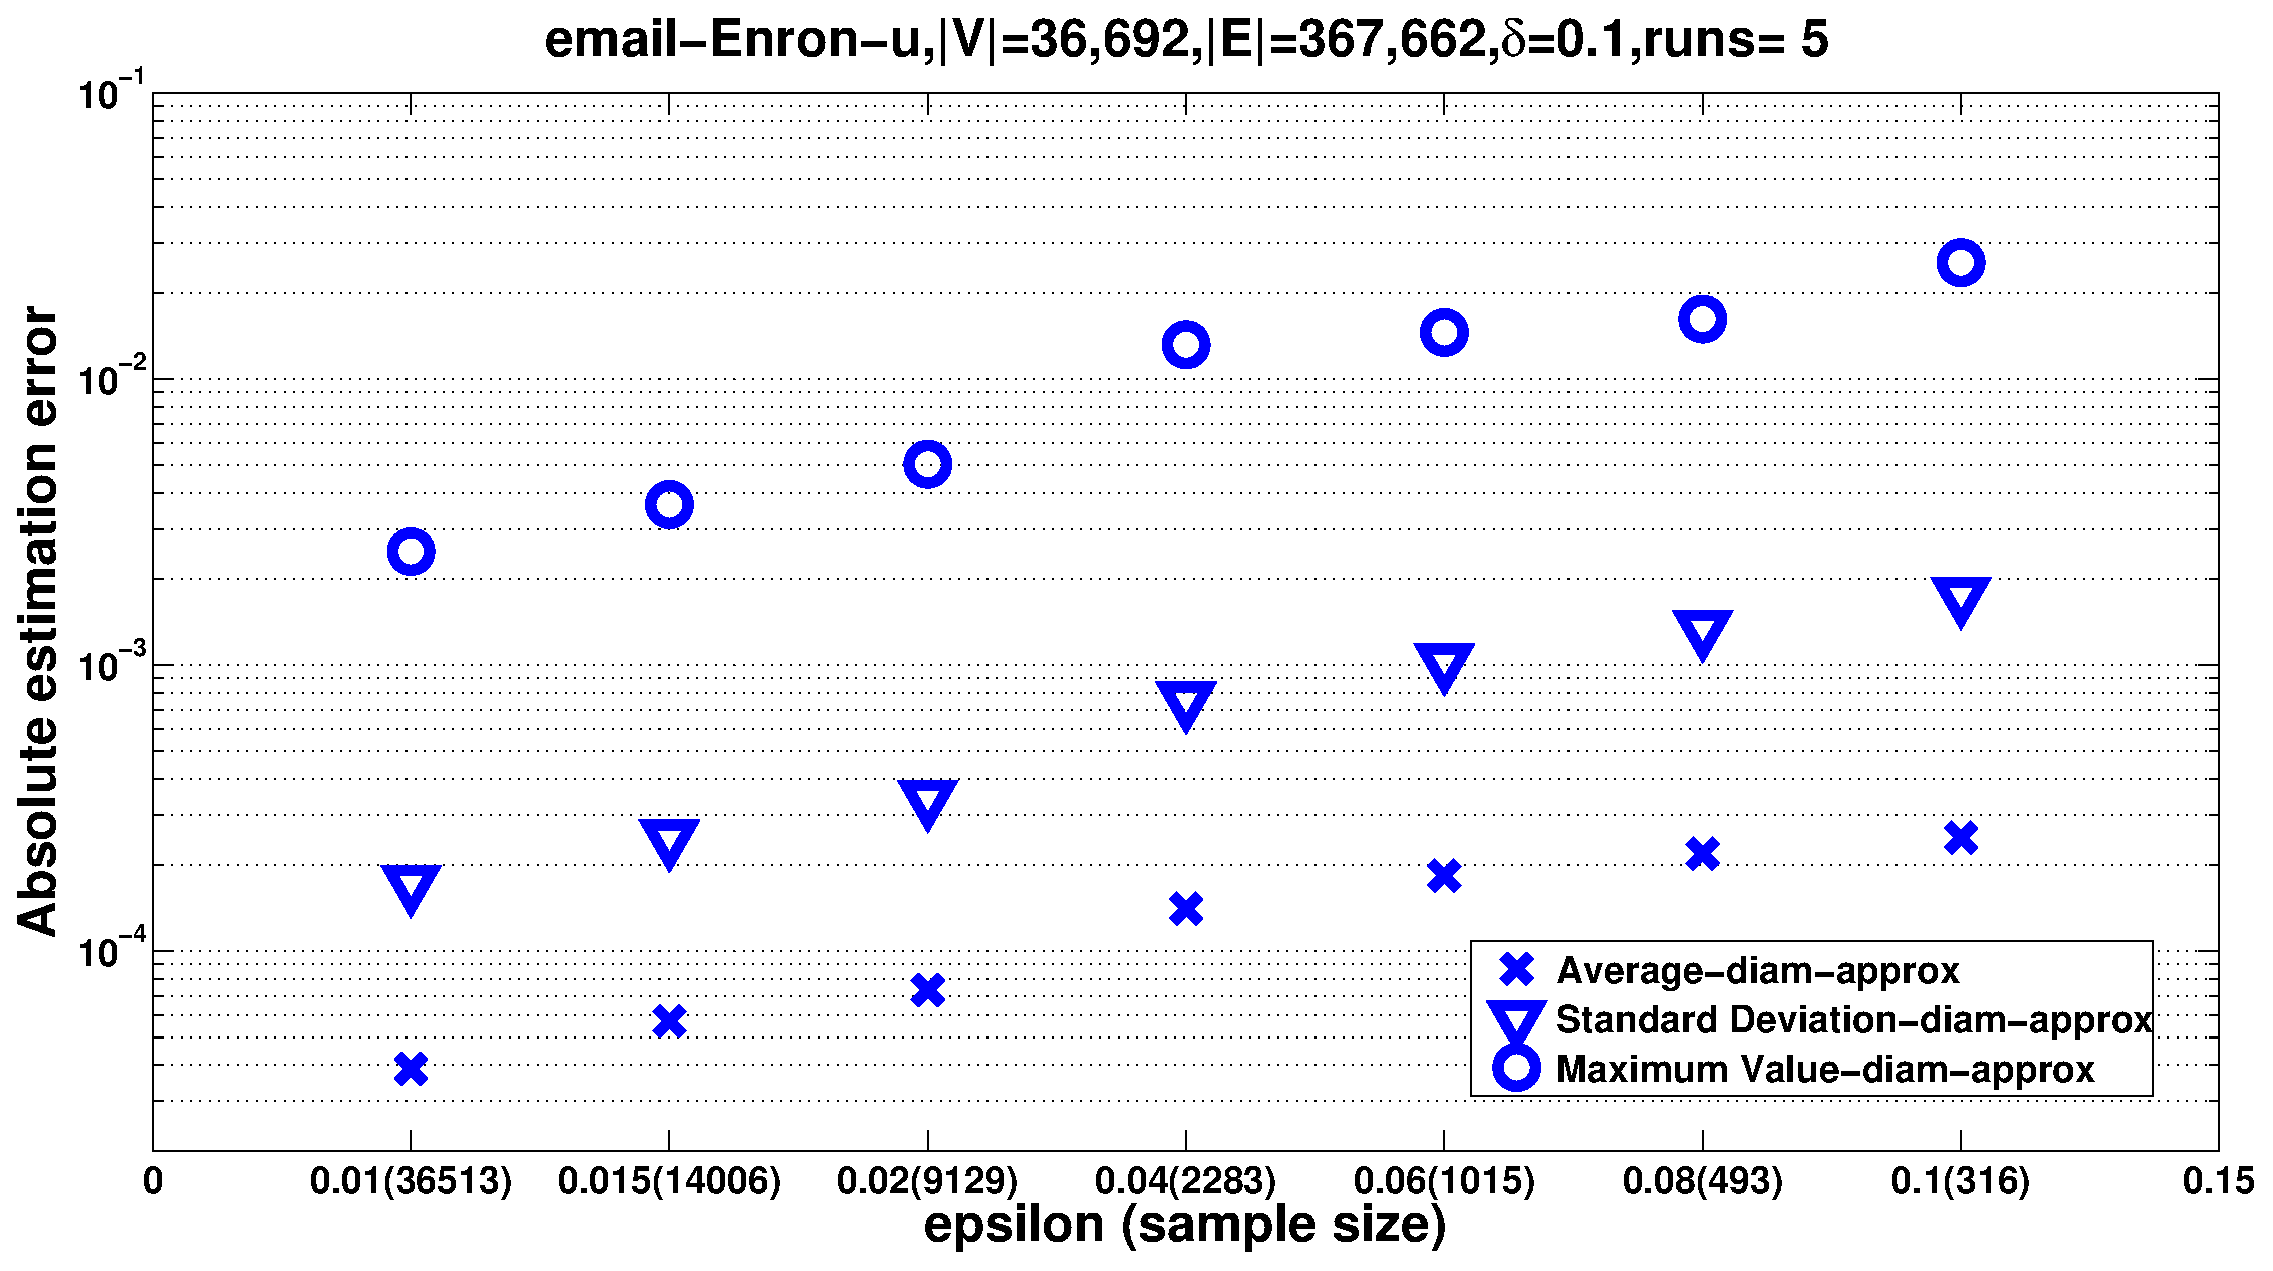
\includegraphics[width=3.8in, keepaspectratio]{email-Enron-error.eps}
%\caption{Error evaluation on email-Enron} \label{fig:email:error}
%\end{minipage}
\end{figure*}

\subsection{Runtime}\label{sec:runtime}
We use two metrics in order to measure the amount of computations that the
algorithms perform. The first metric is the execution time, or \textit{time}, in
seconds, the second metric is the number of edges that the algorithm
touched/traversed, or \textit{touched edges}, during the execution. The number
of touched edges is a graph theoretic metric \XXX What do you mean by that? that
does not depend on the specifications of the implementation environment and
gives a perspective of the amount of work that the algorithm requires. It is
worth mentioning that we count an edge as many times as it is touched during
a run of an algorithm, so we might count a single edge more than once. The
algorithms take parameters $\varepsilon$ and $\delta$ and compute the sample
size accordingly. For our experiments we used $\delta=0.1$, while $\varepsilon$
takes value in $\{0.01, 0.015, 0.02, 0.04, 0.06, 0.08, 0.1\}$. We run each
experiments five times for each value of $\varepsilon$, and measured the average
running time as well as the average number of touched edges. 
The results are presented in~\cref{tab:expUndir,tab:expDir}
and~\cref{fig:gnutella:time,fig:gnutella:edges,fig:email:time,fig:email:edges}.
We denote our algorithm with $\mathsf{VC}$ and the one from~\citep{BrandesP07}
with $\mathsf{BP}$. The performances of the algorithm proposed
in~\citep{GeisbergerSS08} are the same as those of $\mathsf{BP}$, because it
follows the same sampling approach as the one
from~\citep{BrandesP07,JacobKLPT05} and only differs in the definition of the
estimator for the betweenness of a vertex. Because of this, it takes the same
amount of time and touches the same number of edges as the one
from~\citep{BrandesP07}.

In~\cref{tab:expUndir}, for each of
the 7 values of $\varepsilon$, we present the minimum and maximum ratio of the
average touched edges of $\mathsf{BP}$ over $\mathsf{VC}$, as well as the
minimum and maximum ratio of the average running time %of BP over VC. 
As it can be seen from this table our algorithm performs significantly faster,
more than 300\%, in both measures. In~\cref{tab:expDir} we compare the
algorithms on a set of directed graphs. As in the case of the undirected graphs,
we present the minimum and maximum ratios of corresponding measures for the
different values of $\varepsilon$. From the table we can see
that the value for the vertex-diameter that we consider in the case of diam-UB
is many orders of magnitudes greater than the actual value, which translates in
a significant increase of the number of samples. But even in the case of this
crude vertex-diameter approximation (diam-UB), the $\mathsf{VC}$ algorithm
performs uniformly faster than $\mathsf{BP}$. In the case where the exact value
of the diameter was used, we can see that our algorithm computes an estimation
of the betweenness that satisfies the desired accuracy and confidence guarantees
\emph{3 to 5 times faster} than~\citep{BrandesP07}. \XXX-(COMMENT ON THE
RELATION TOPOLOGY-SPEED) 

In~\cref{fig:gnutella:time} we study the directed graph \texttt{p2p-Gnutella30}
and we present the measurements of the average running time of the algorithms in
a logarithmic scale, using the exact algorithm from~\citep{Brandes01} as
baseline. The $\mathsf{VC}$ algorithm requires significantly less time
than the $\mathsf{BP}$algorithm. The diam-UB and the diam-exact can be seen as
the two extremes for the performance of our algorithm in terms of time. In the
case of the diam-exact we have as few samples as possible since we use the exact
value of the vertex-diameter, whereas in the case of diam-UB we have as many
samples as possibles since we use the worst case estimation for the
vertex-diameter of the graph. 
%(that is when the graph has a hamiltonian path) <= not correct.
In~\cref{fig:email:time} we study the average running time of the algorithms for
the undirected graph \texttt{email-Enron}. In this case our algorithm not only
performs better but also \emph{scales} better than the one
from~\citep{BrandesP07} \XXX WHAT DO YOU MEAN SCALES BETTER?. 
%For the computation of the sample size we use the 2-approximation algorithm
%which is enough since what we really use for the computation of sample size is
%the logarithm of the diameter. 
In~\cref{fig:gnutella:edges,fig:email:edges}, we study the average number of
touched edges for the case of the directed graph \texttt{p2p-Gnutella30} and of
the undirected graph \texttt{email-Enron} respectively. It is evident that again
our algorithm outperforms $\mathsf{BP}$. 

From the above Figures and Tables we see that for the tested values of
$\varepsilon$, the proposed algorithm is faster(at least 3x speedup in case of
exact diameter on the tested graphs) and requires less amount of work(at least
3x speed up on the tested graphs) \XXX FASTER THAN WHAT?. The reason is twofold
and it is due to our novel analysis using the VC-dimension: 1) we use a
significantly smaller amount of samples and B) only in the
worst case  we do the same amount of computations per sample as
the state of the art, as our algorithm needs to find the shortest path between a
sampled pair of vertices whereas both 
algorithms from~\citep{GeisbergerSS08,BrandesP07}  need to compute the shortest
paths between a sampled source and all the rest of the nodes.

\XXX Mention bidirectional search and the improvements it can give us.

\begin{figure*}[ht]
  \centering
  \hfill
  \subfloat[p2p-Gnutella30
  (directed)]{\label{fig:gnutella:time}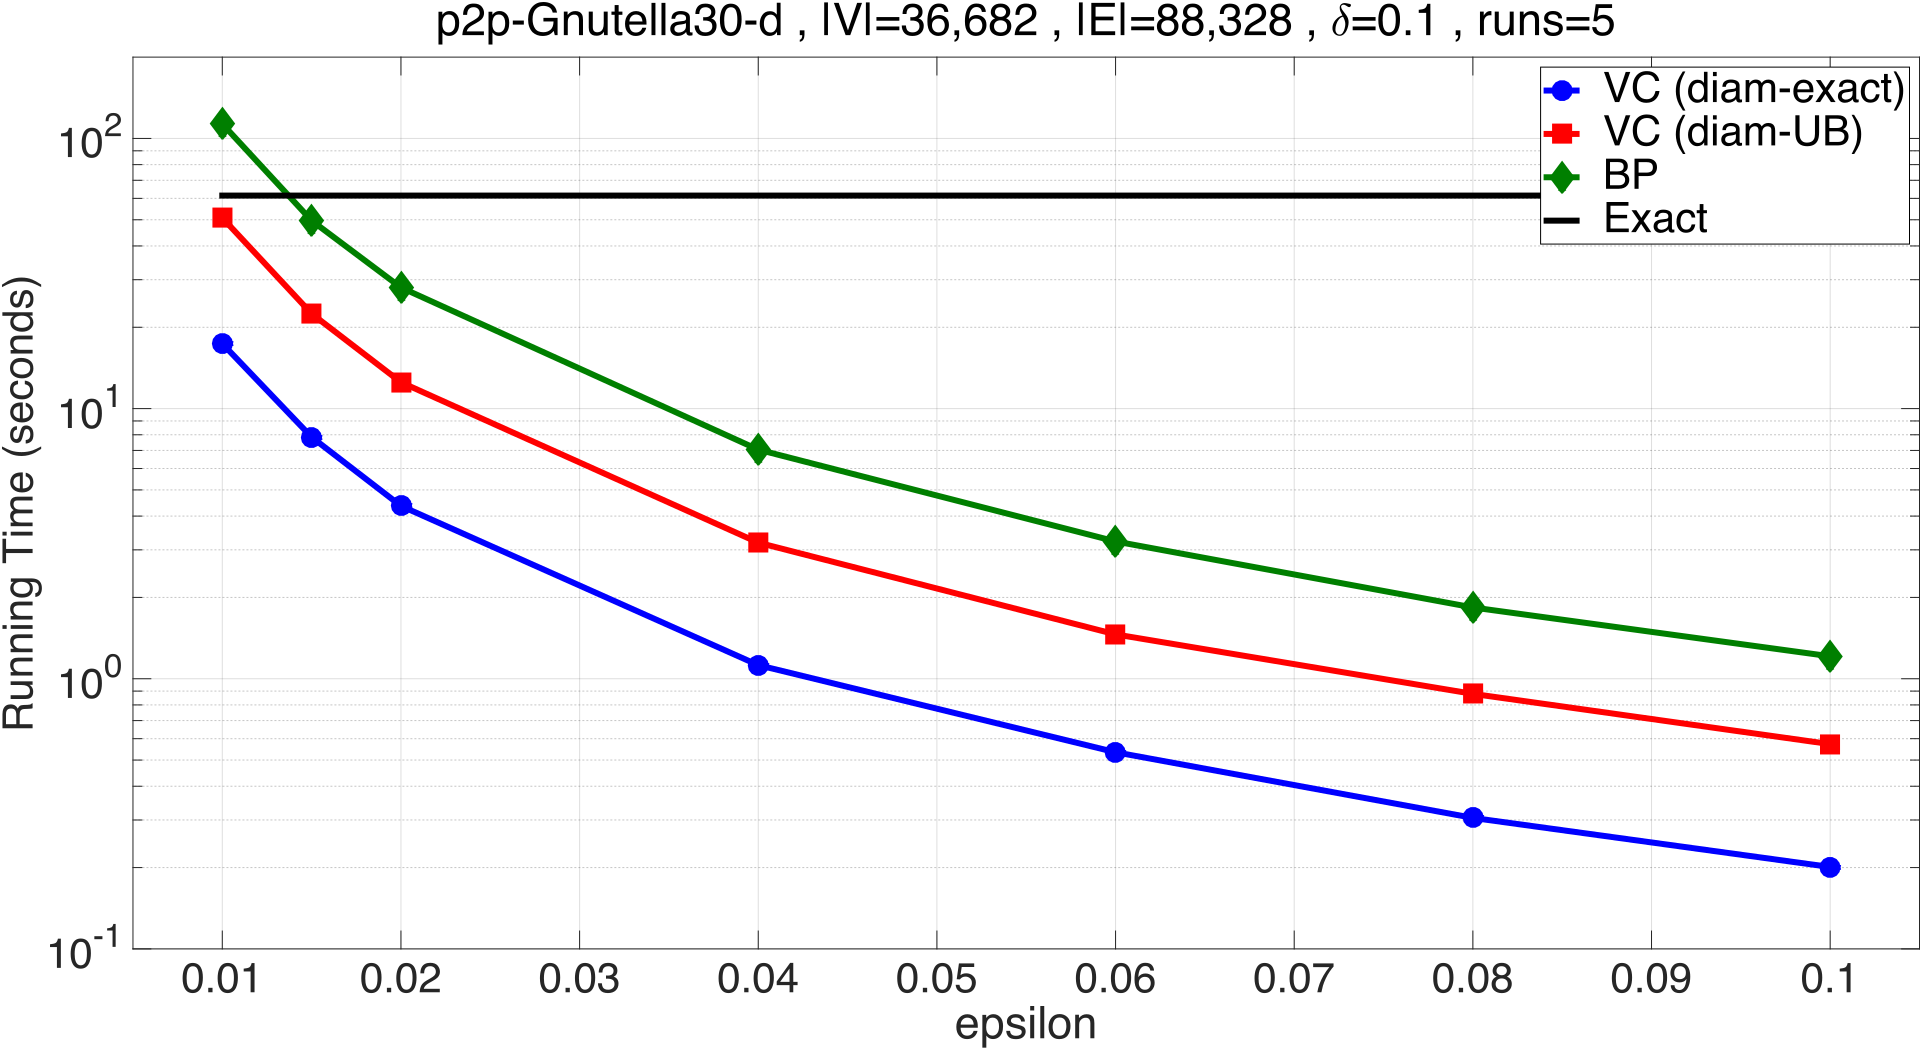
\includegraphics[width=.45\textwidth,keepaspectratio]{p2p-Gnutella30-time}}
  \hfill
  \subfloat[email-Enron
  (undirected)]{\label{fig:email:time}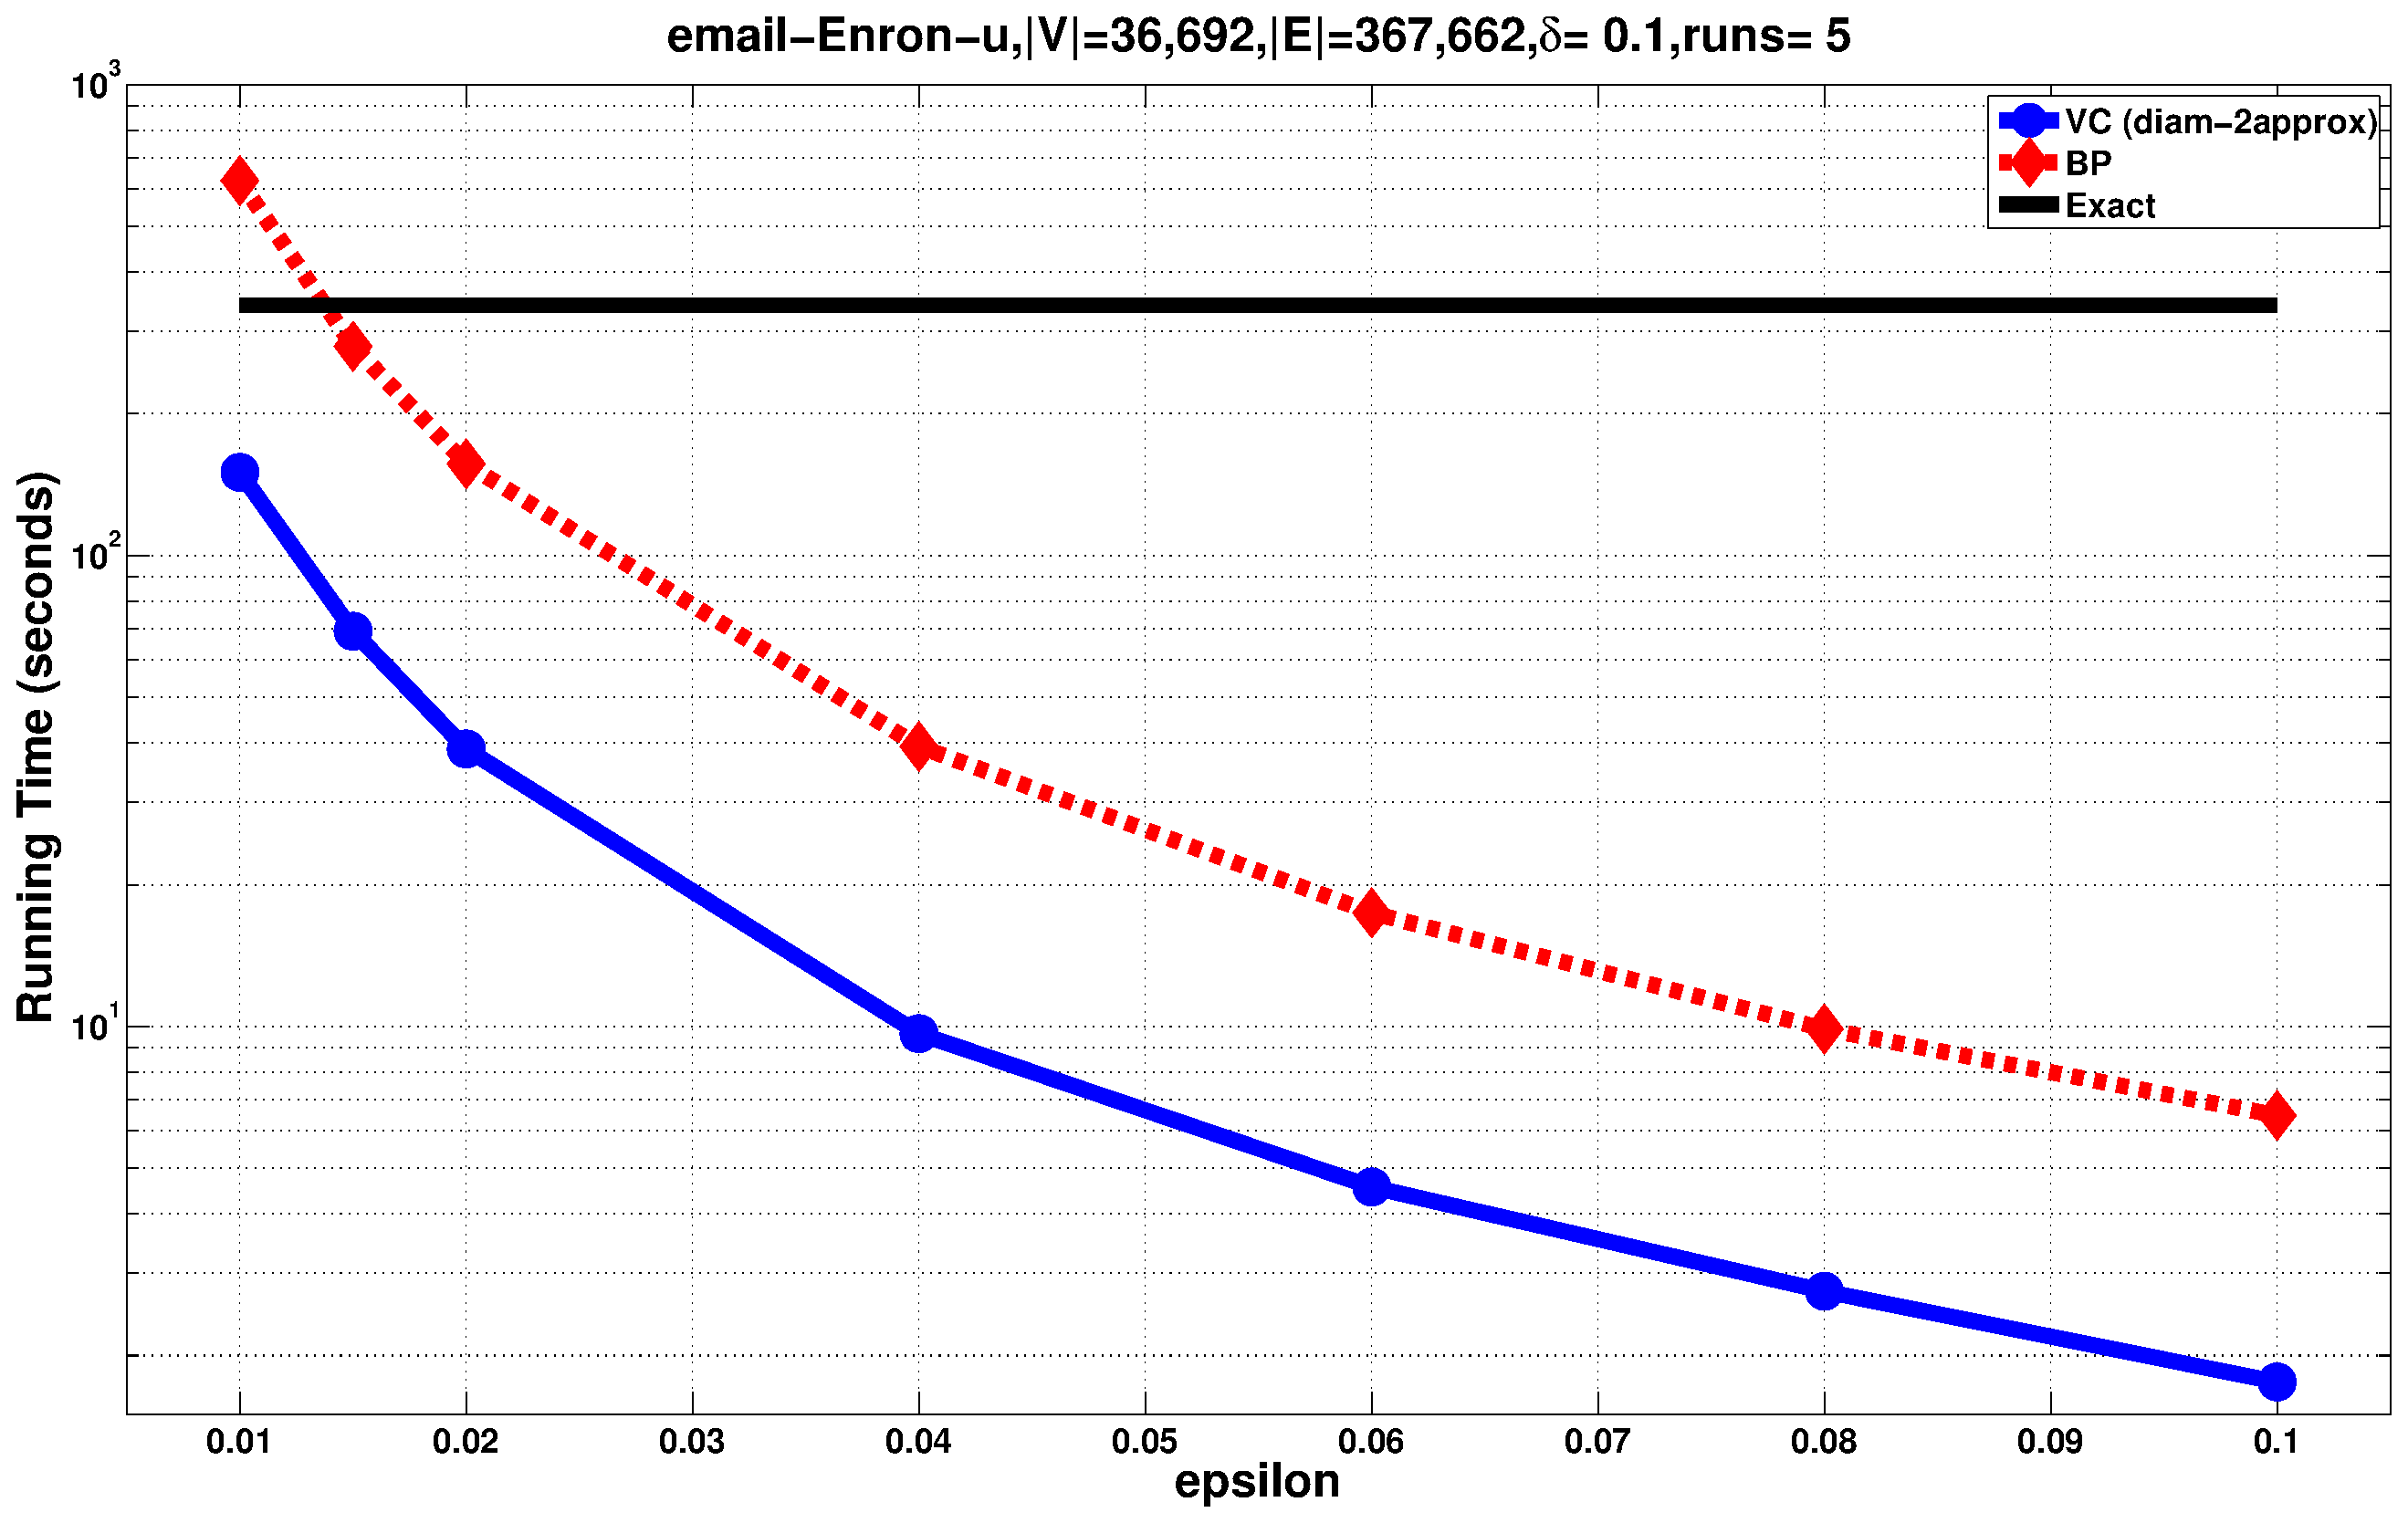
\includegraphics[width=.45\textwidth,keepaspectratio]{email-Enron-time}}
  \label{fig:time}
  \caption{Running time comparison between $\mathsf{VC}$, $\mathsf{BP}$, and the
  exact algorihtm.}
%\begin{minipage}[b]{0.5\linewidth}
%\flushleft
%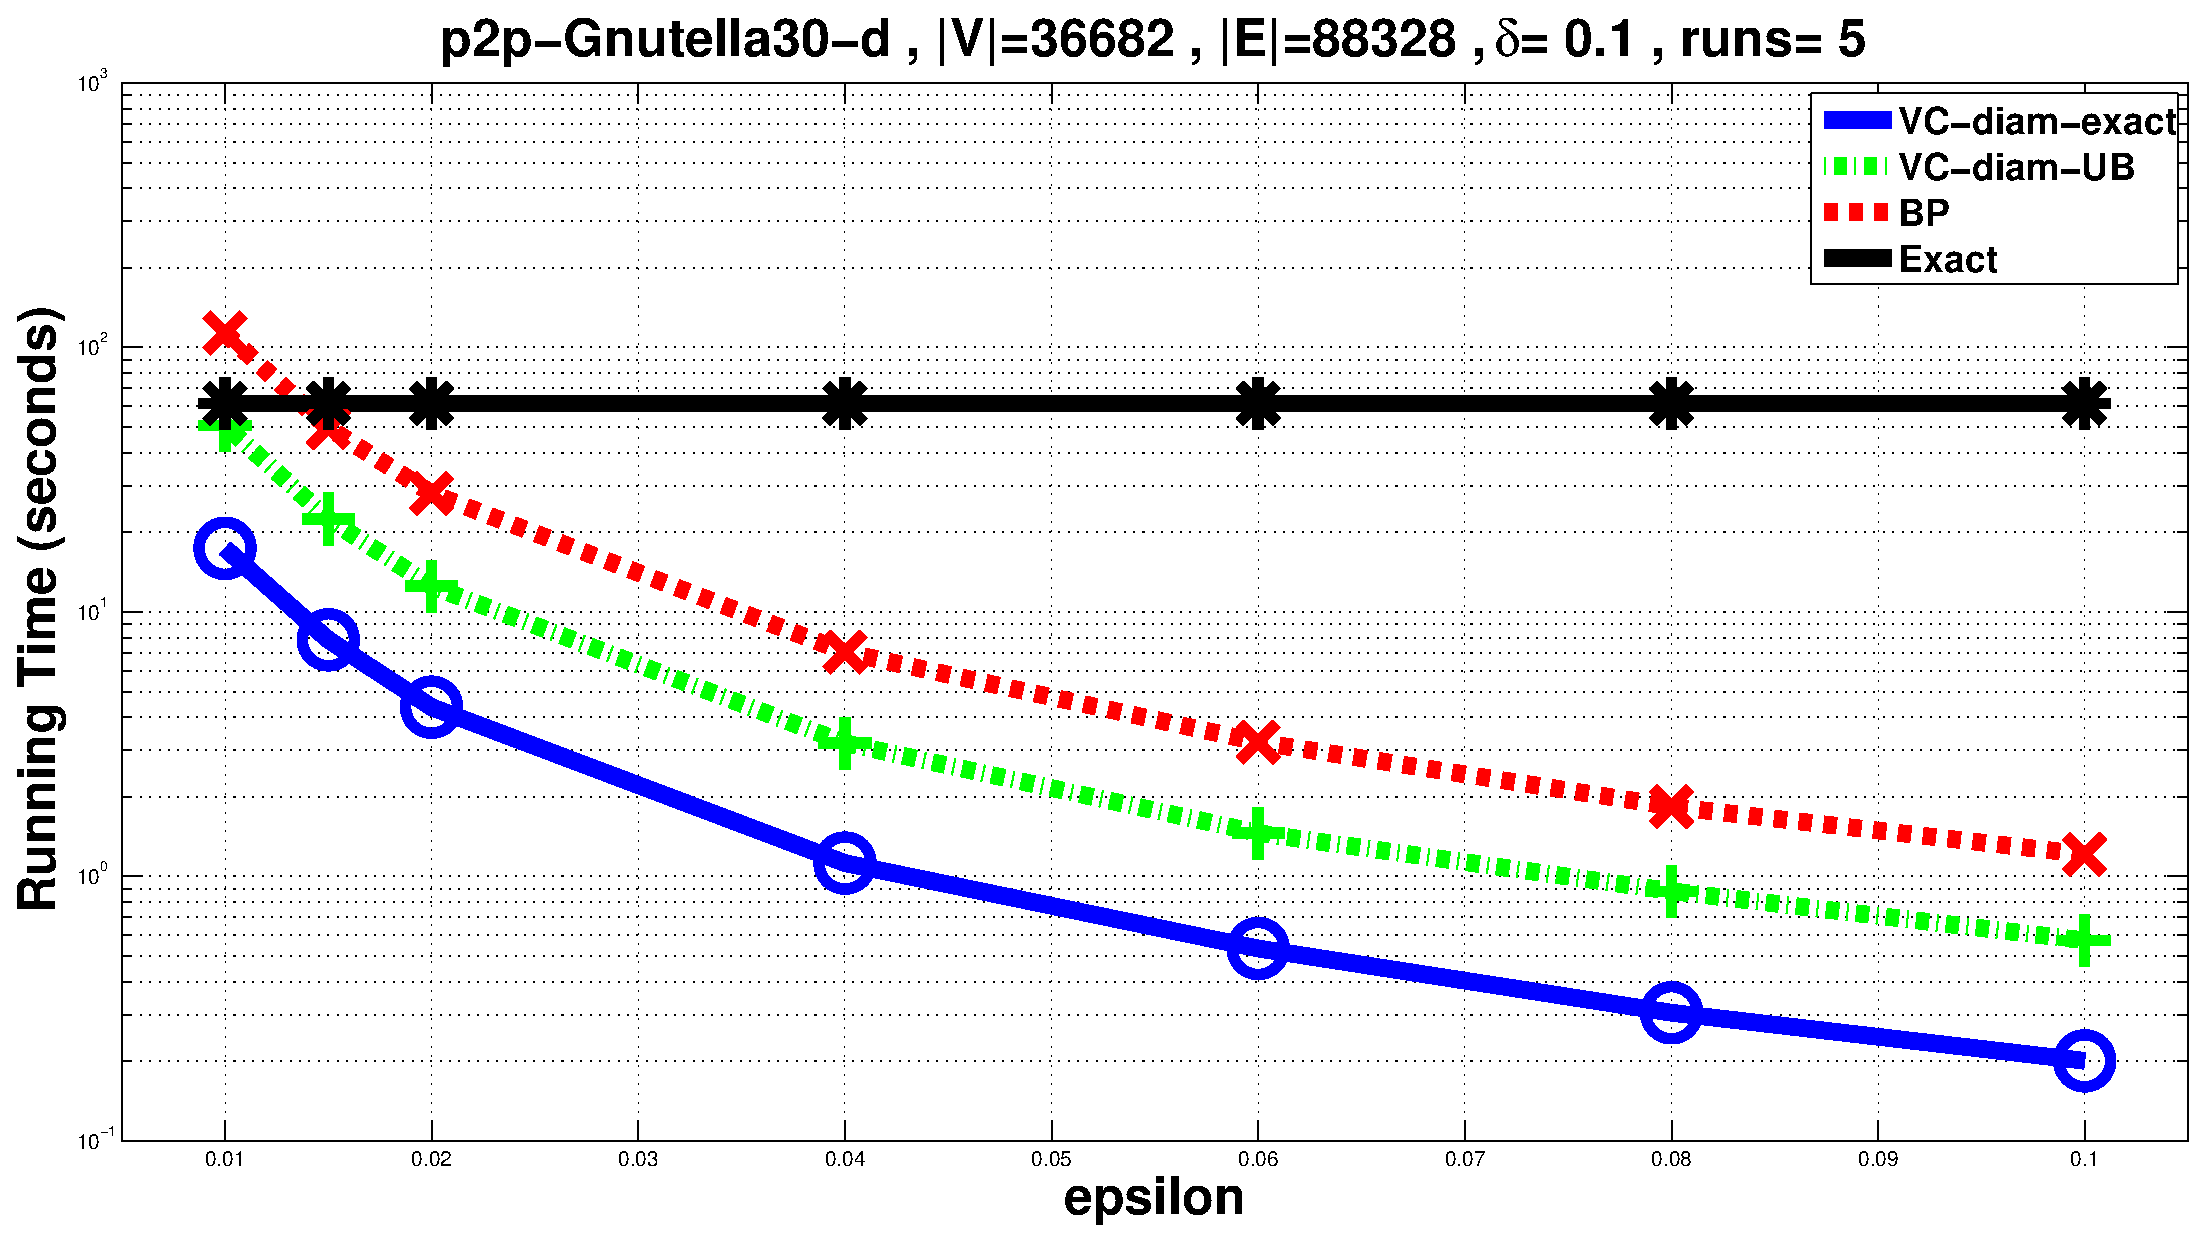
\includegraphics[width=3.8in, keepaspectratio]{p2p-Gnutella30-time.eps}
%\caption{Running time comparison on p2p-Gnutella30} \label{fig:gnutella:time}
%\end{minipage}%
%\begin{minipage}[b]{0.5\linewidth}
%\centering
%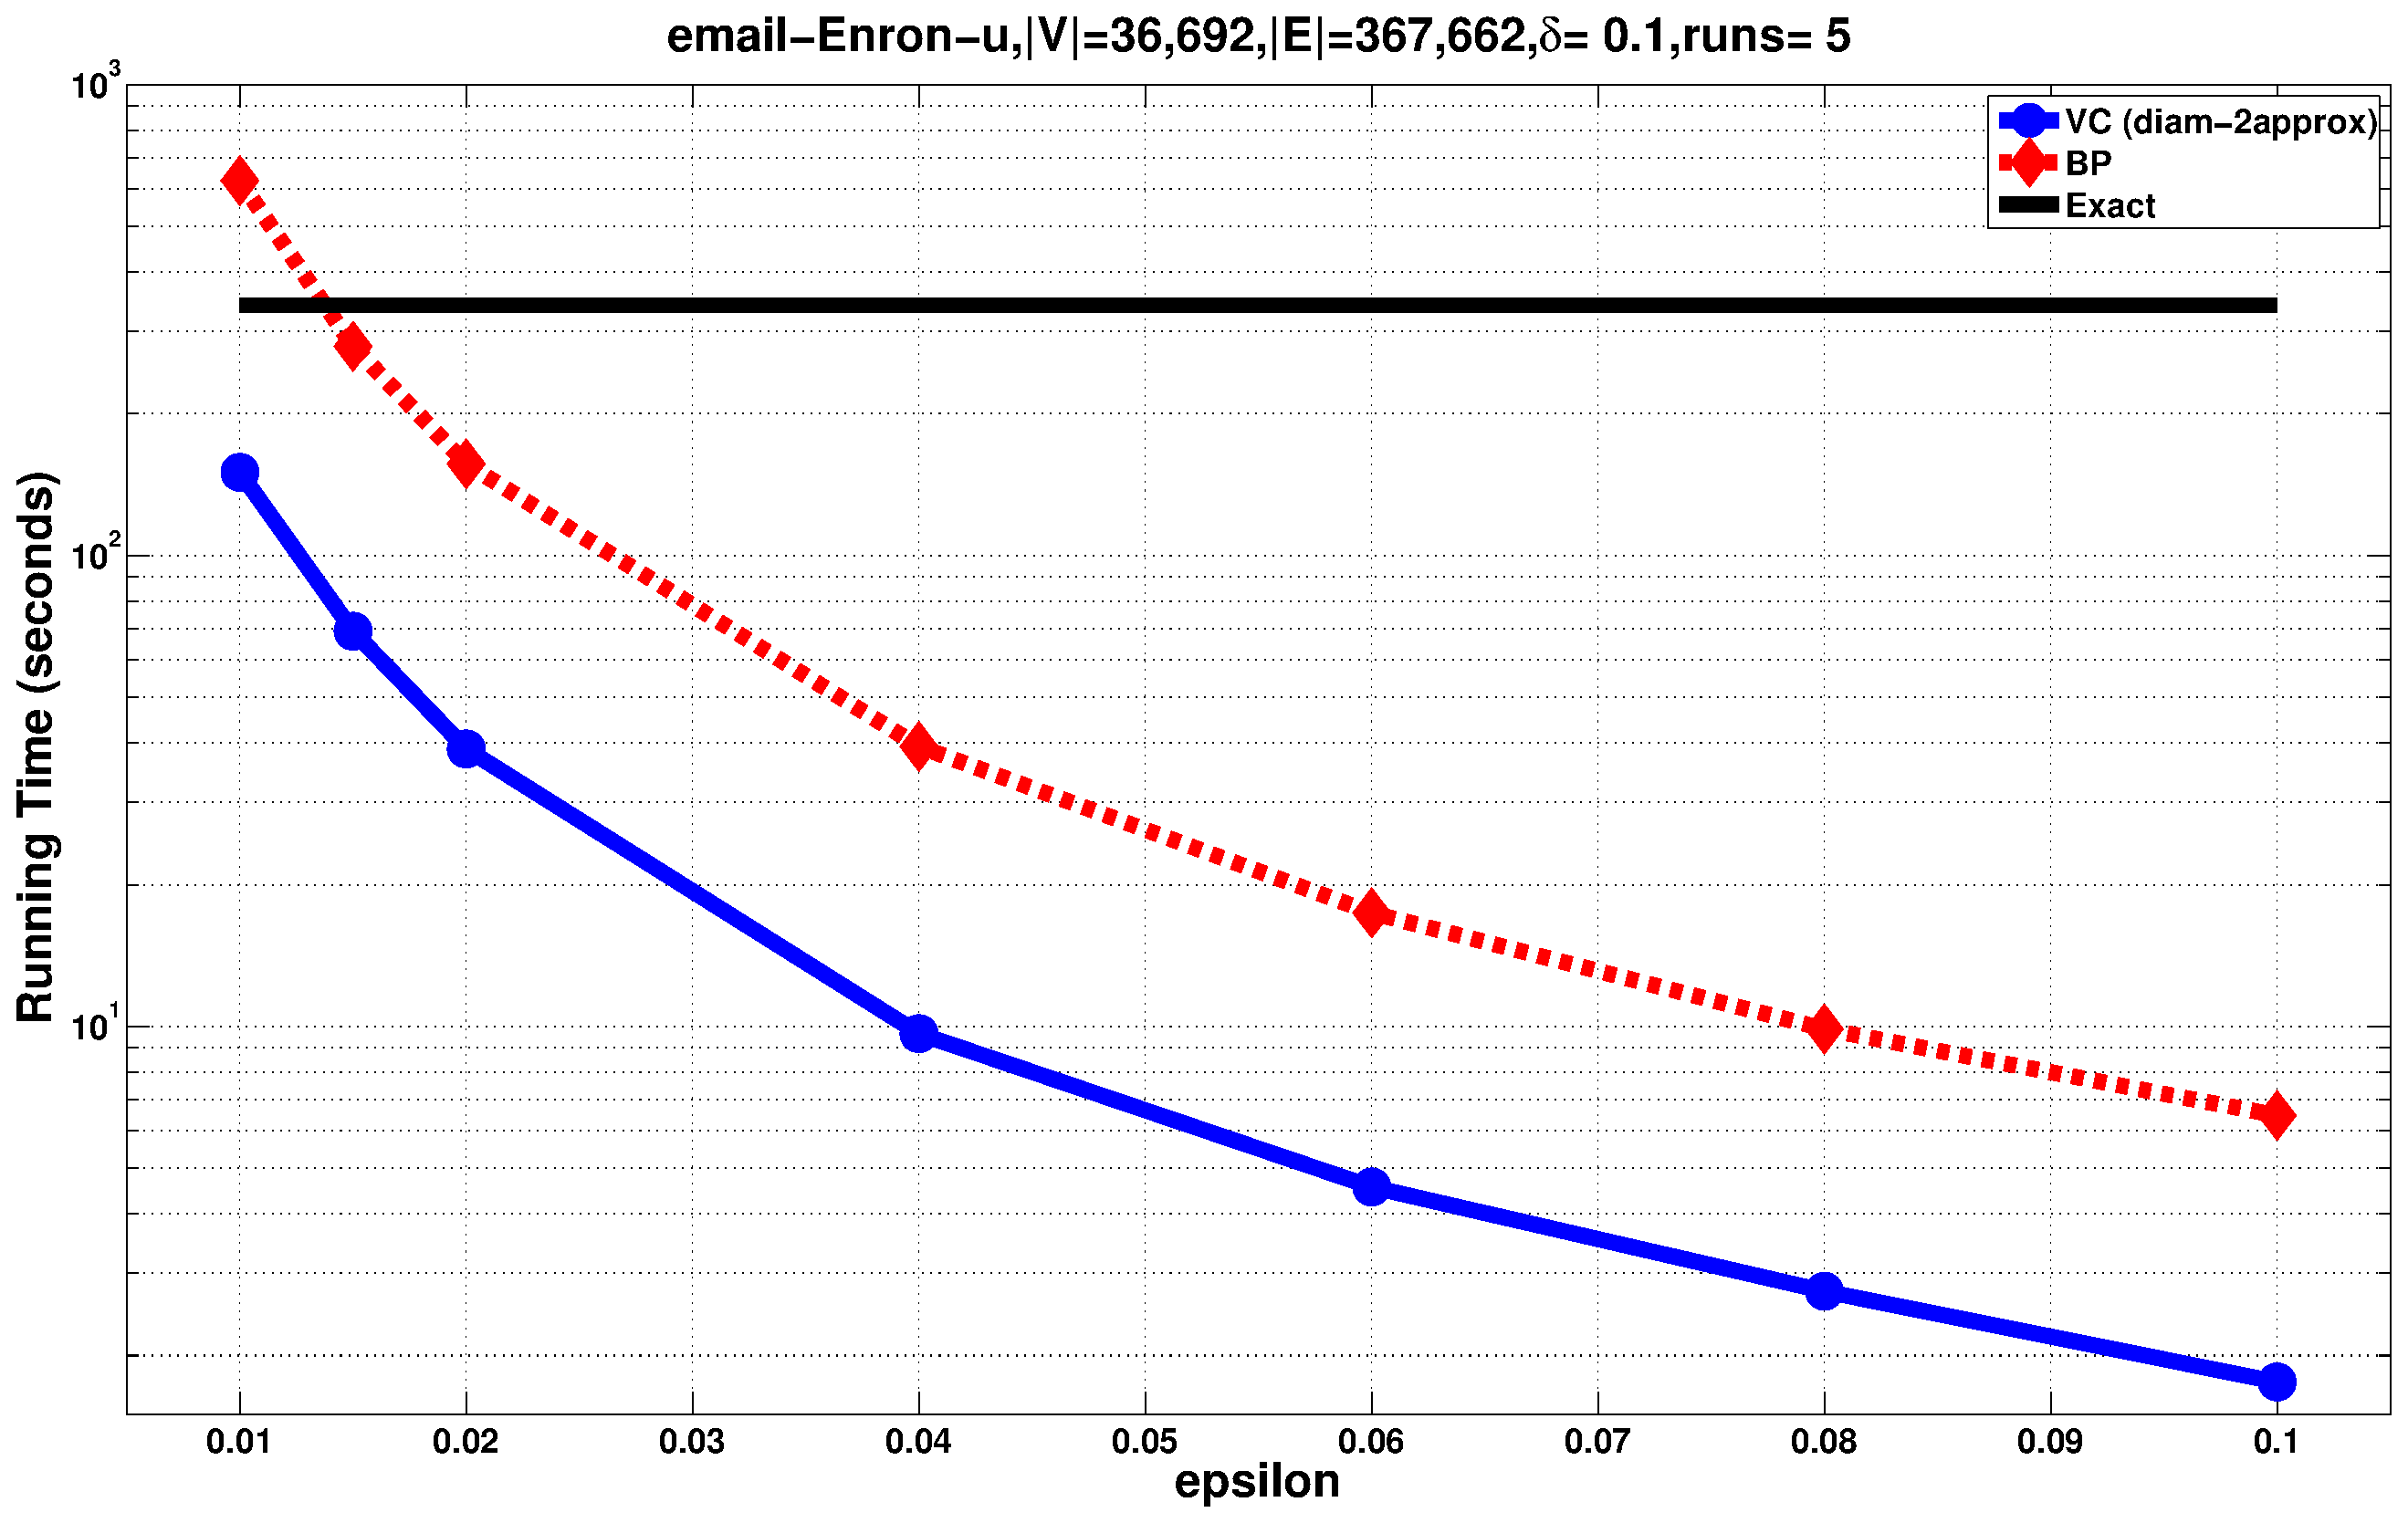
\includegraphics[width=3.8in, keepaspectratio]{email-Enron-time.eps}
%\caption{Running time comparison on email-Enron} \label{fig:email:time}
%\end{minipage}
\end{figure*}


\begin{figure*}[ht]
  \centering
  \hfill
  \subfloat[p2p-Gnutella30
  (directed)]{\label{fig:gnutella:edges}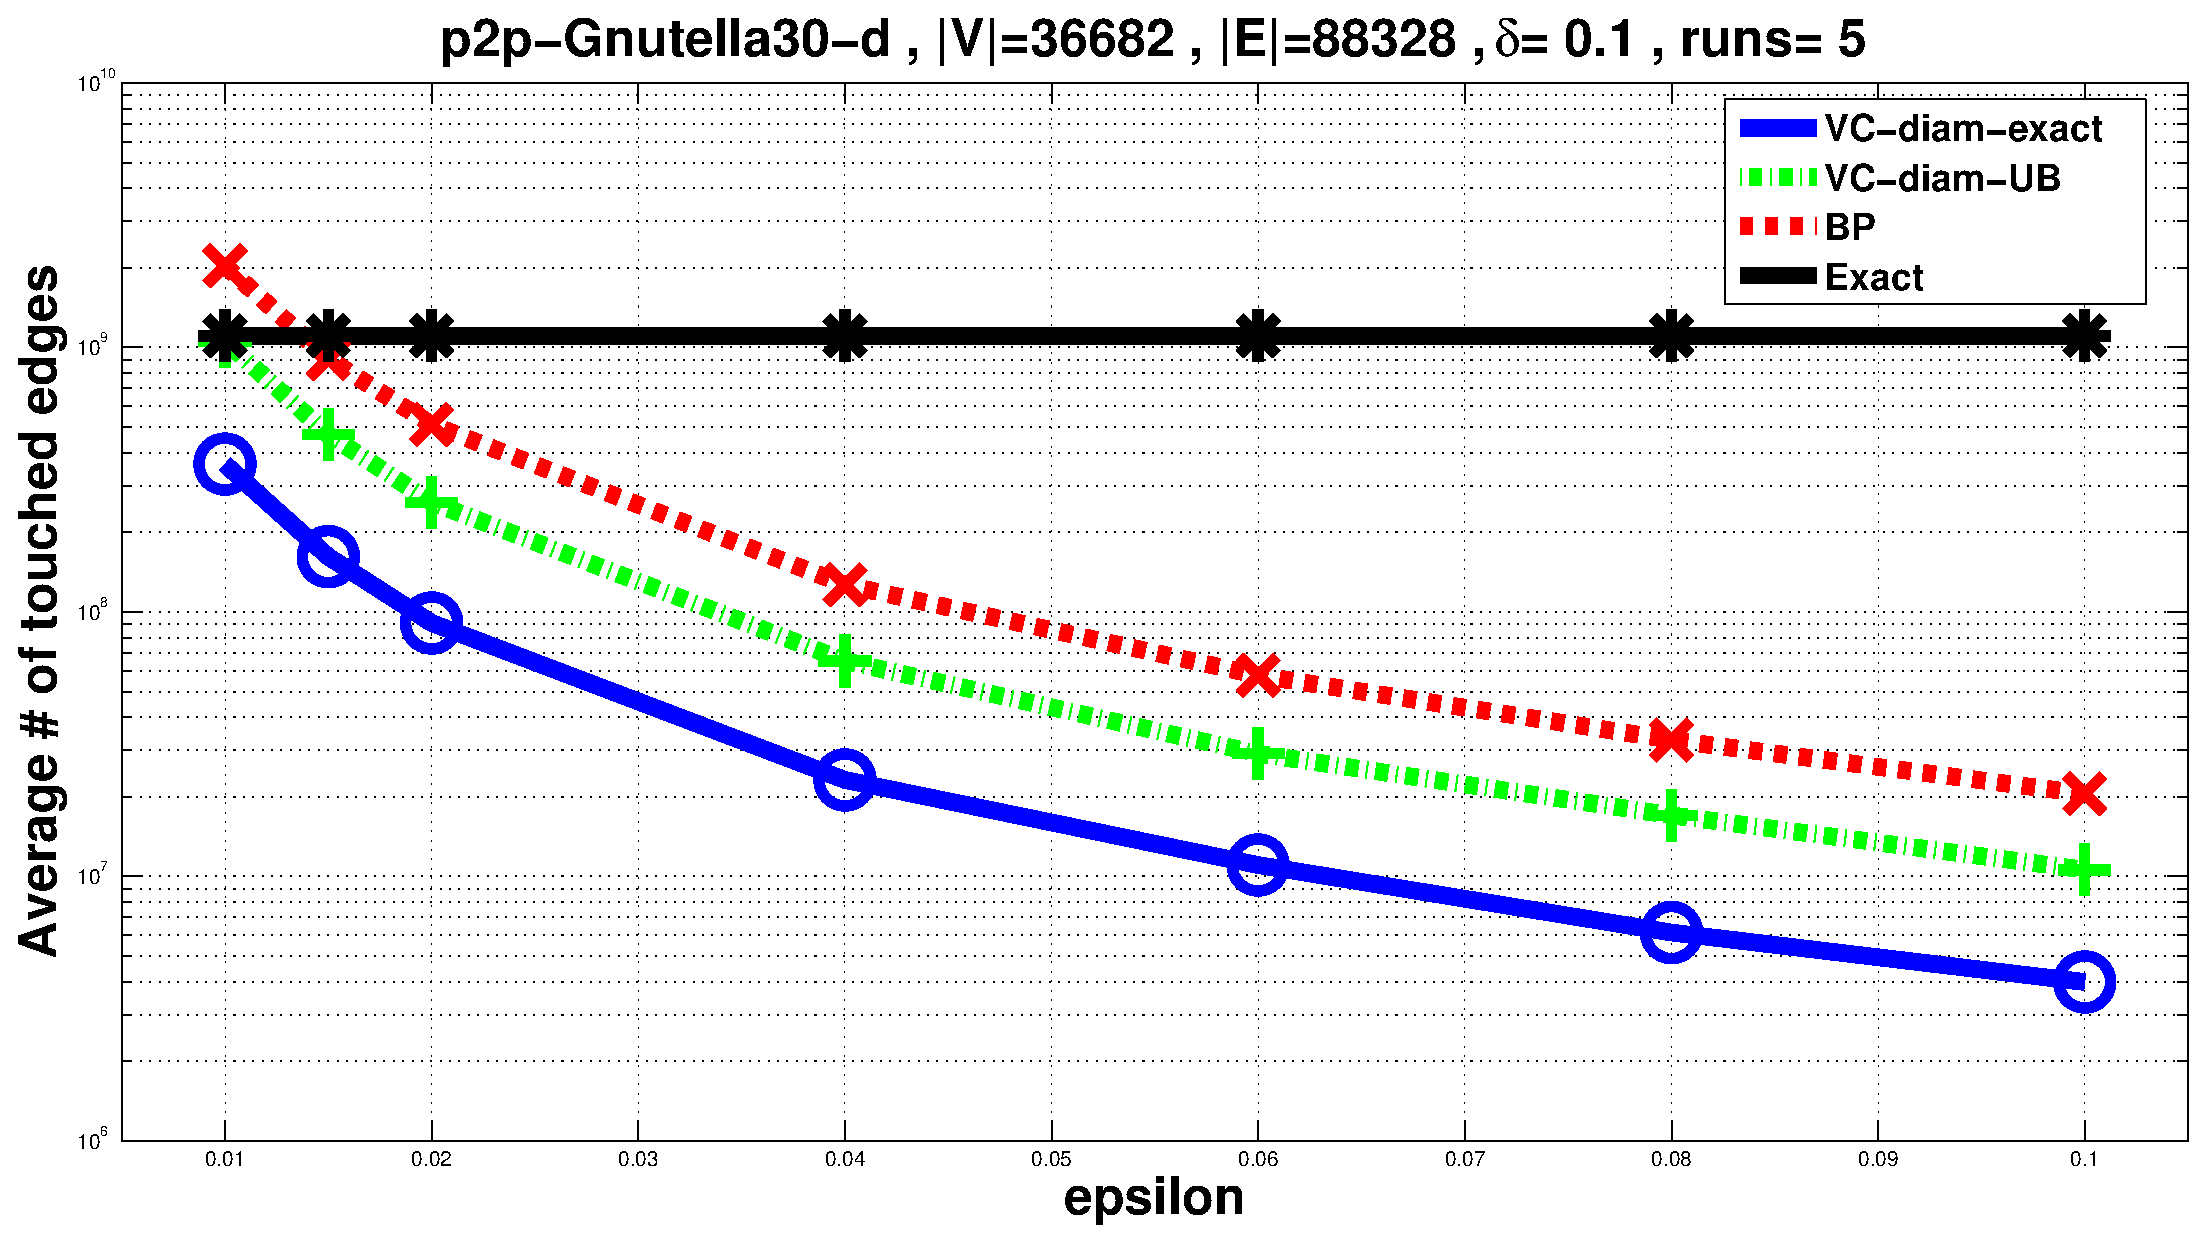
\includegraphics[width=.45\textwidth,keepaspectratio]{p2p-Gnutella30-edges}}
  \hfil
  \subfloat[email-Enron
  (undirected)]{\label{fig:email:edges}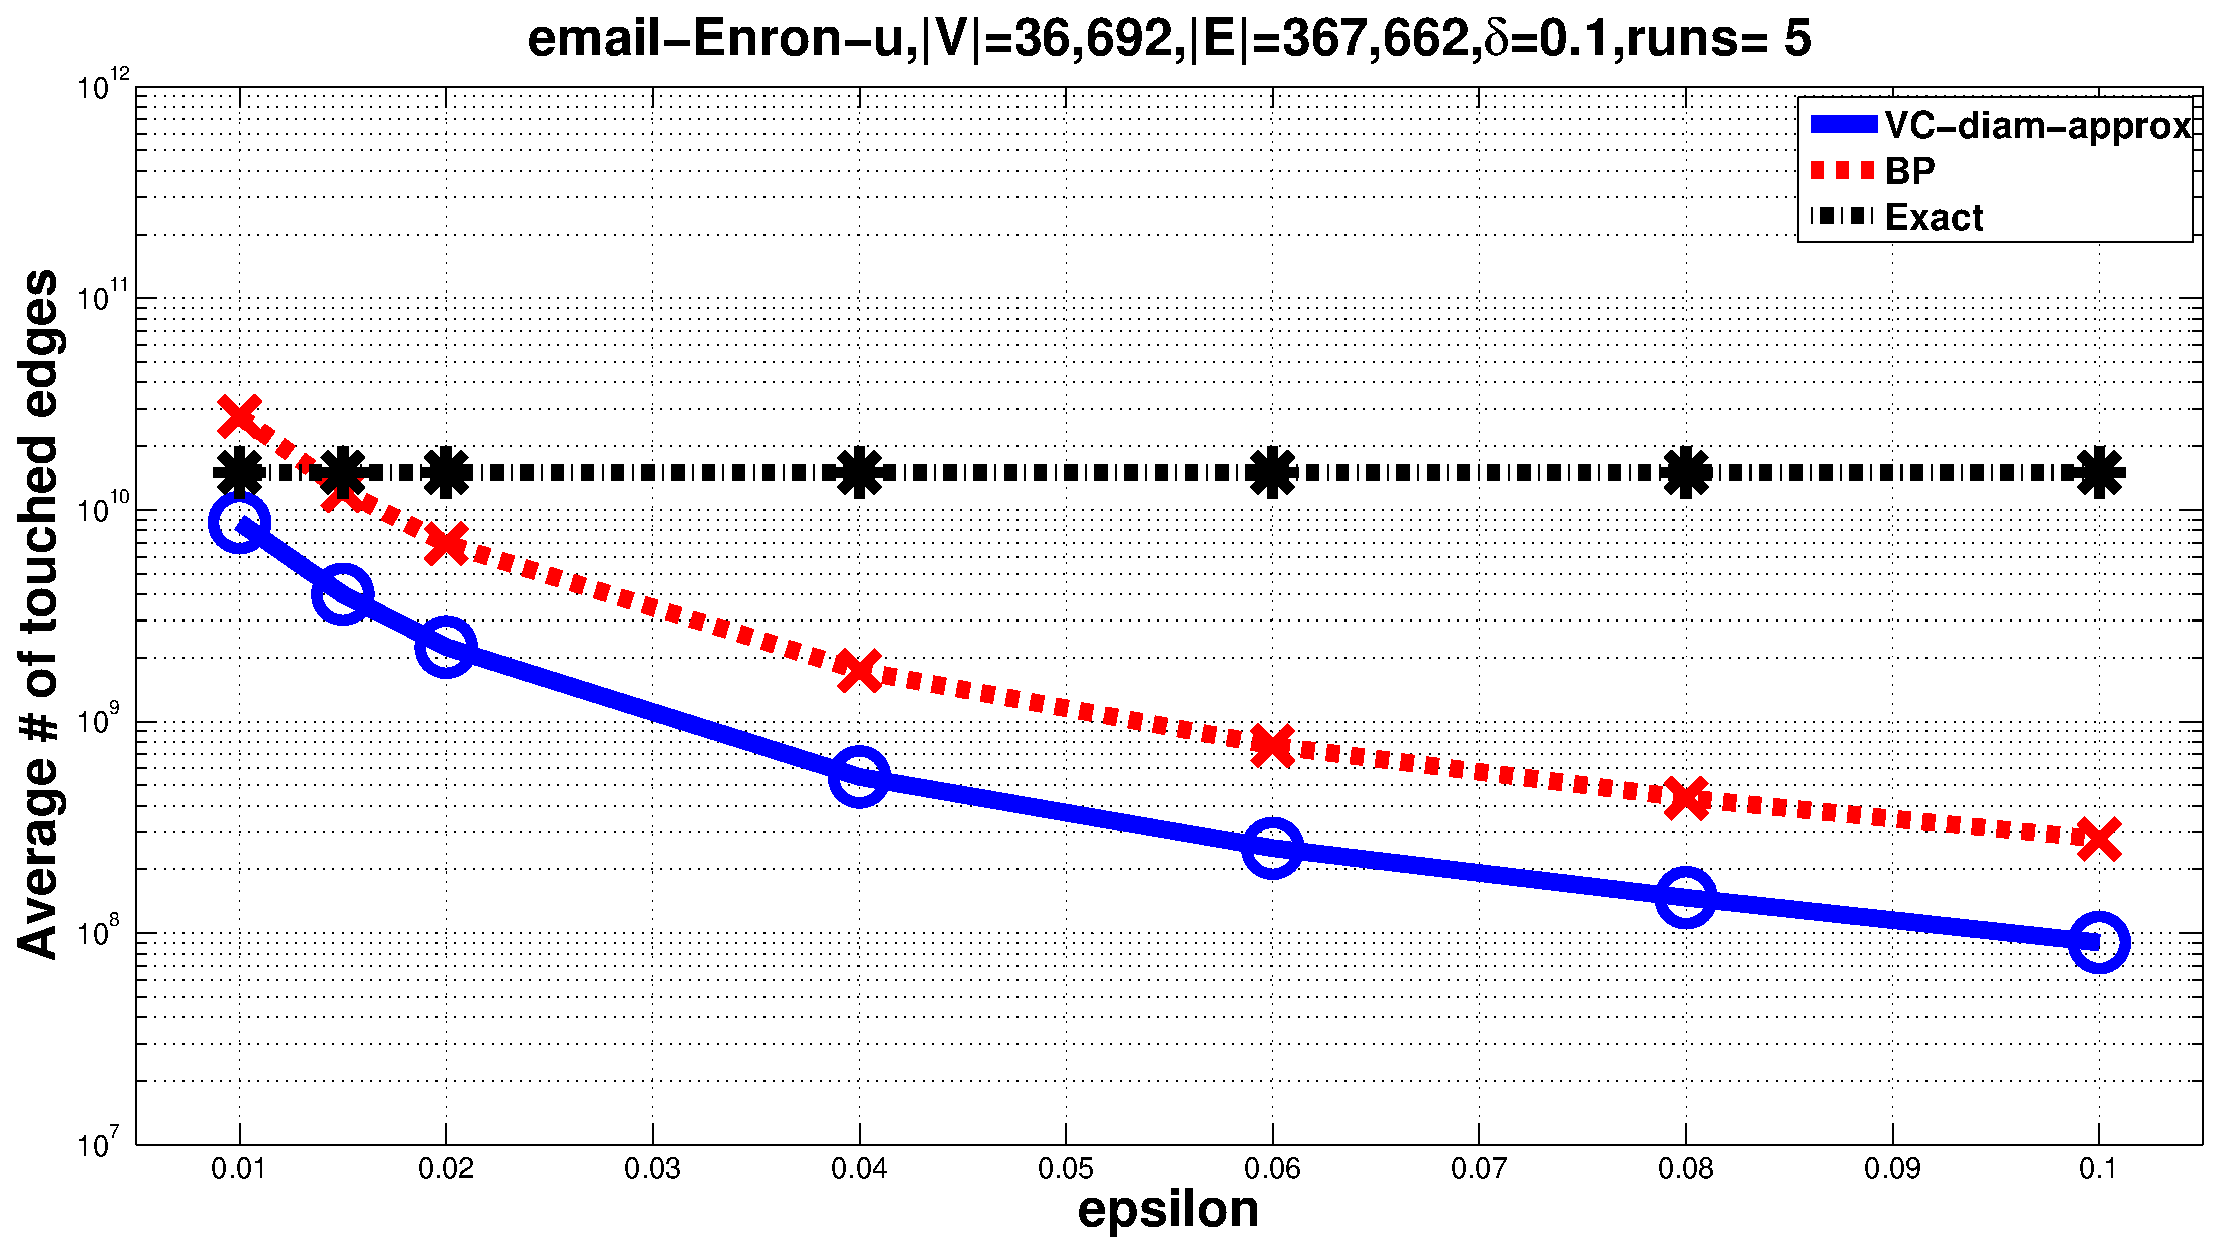
\includegraphics[width=.45\textwidth,keepaspectratio]{email-Enron-edges}}
  \hfill
  \label{fig:edges}
  \caption{Touched edges comparison between $\mathsf{VC}$, $\mathsf{BP}$, and
  the exact algorithm.}
%\begin{minipage}[b]{0.5\linewidth}
%\flushleft
%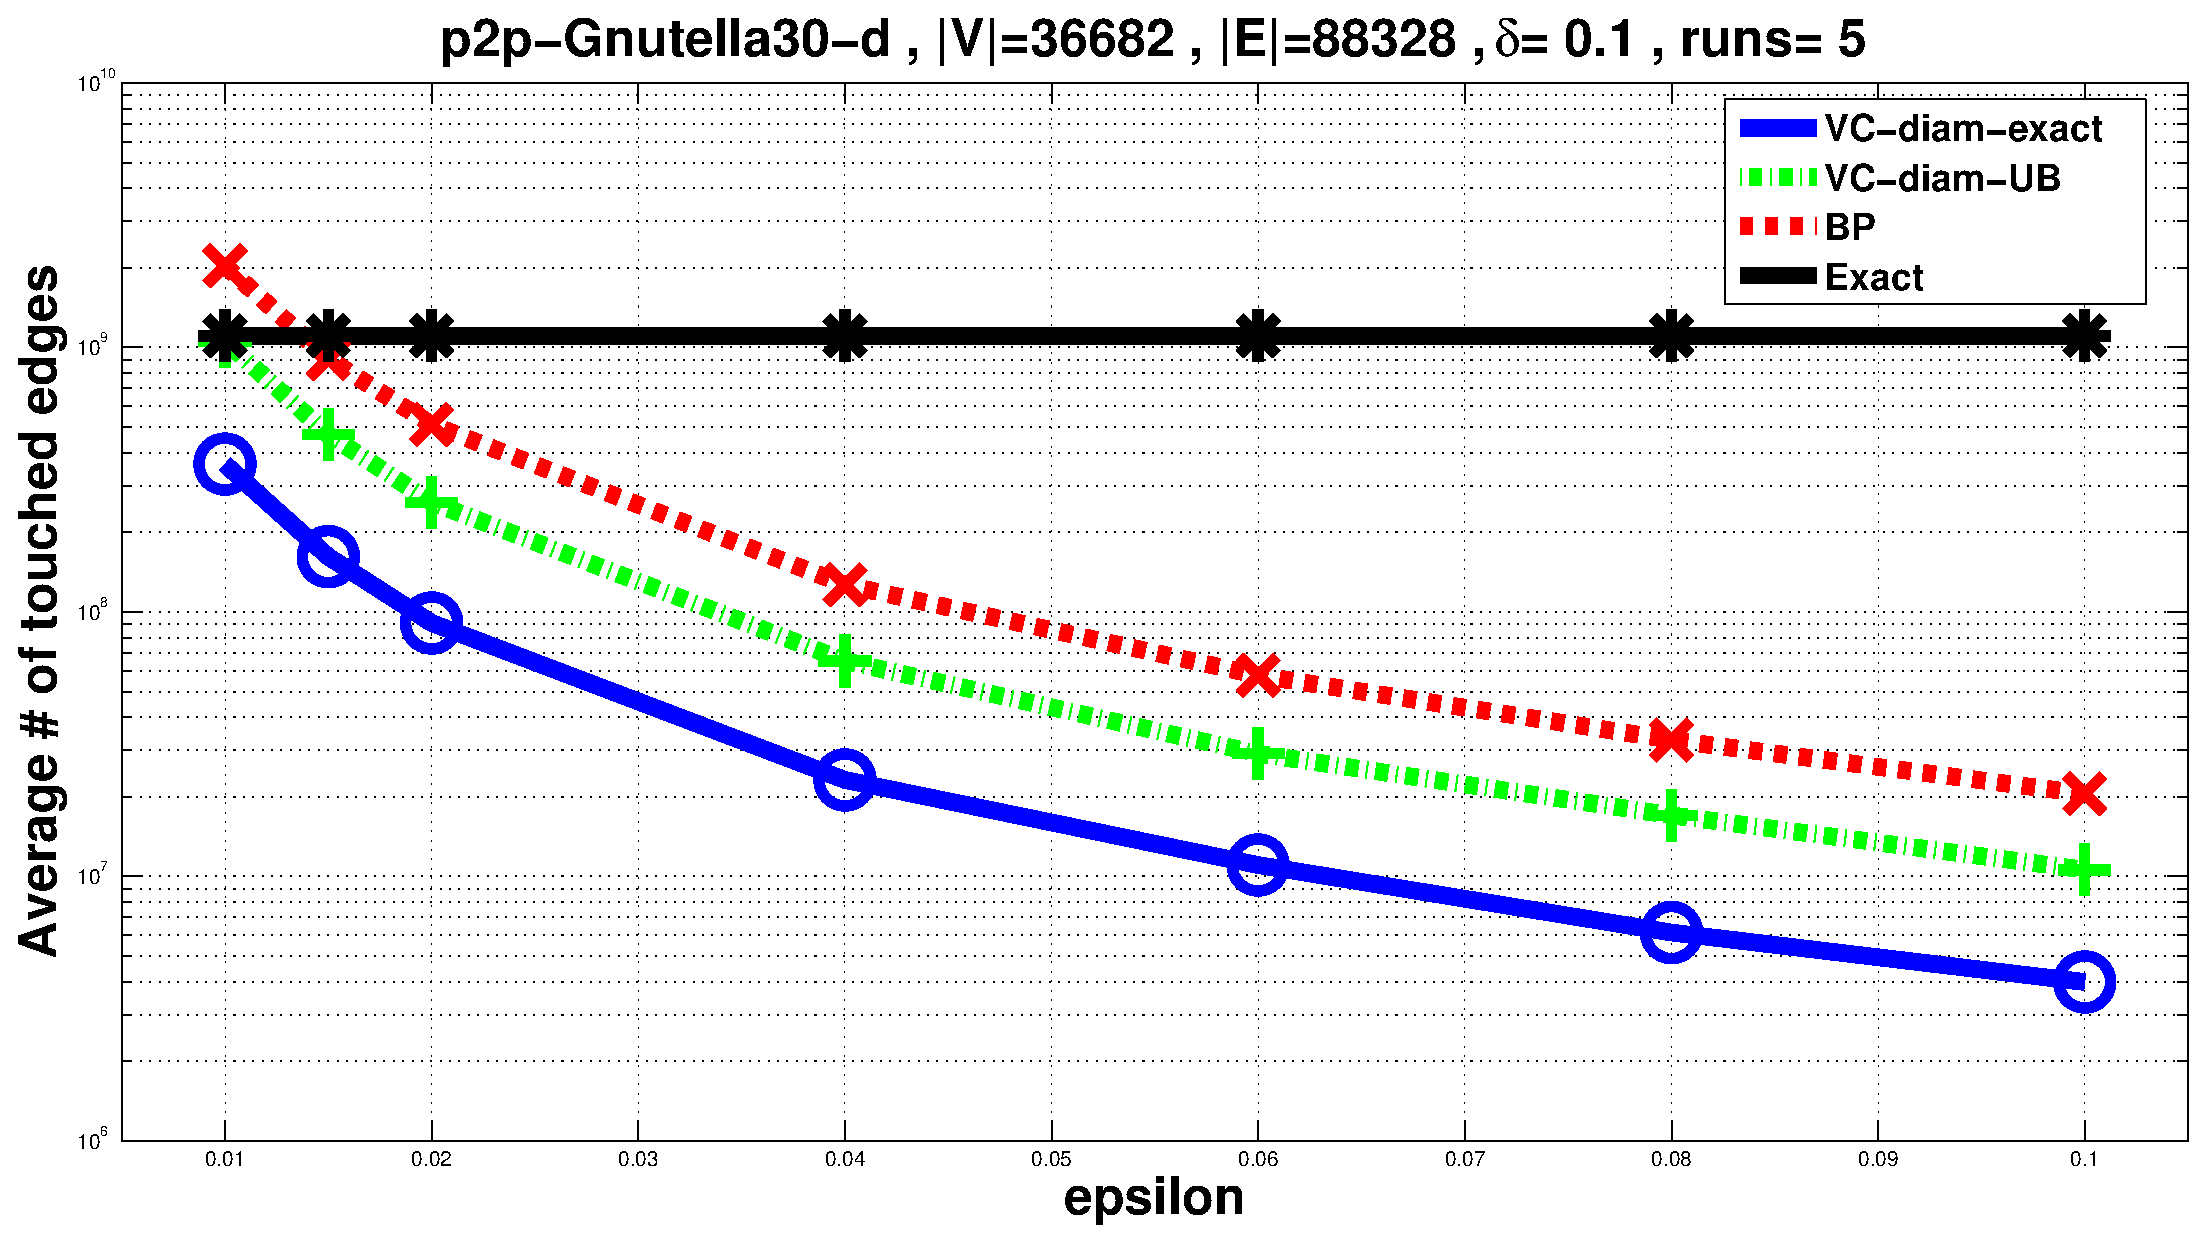
\includegraphics[width=3.8in, keepaspectratio]{p2p-Gnutella30-edges.eps}
%\caption{Touched edges comparison on p2p-Gnutella30} \label{fig:gnutella:edges}
%\end{minipage}%
%\begin{minipage}[b]{0.5\linewidth}
%\centering
%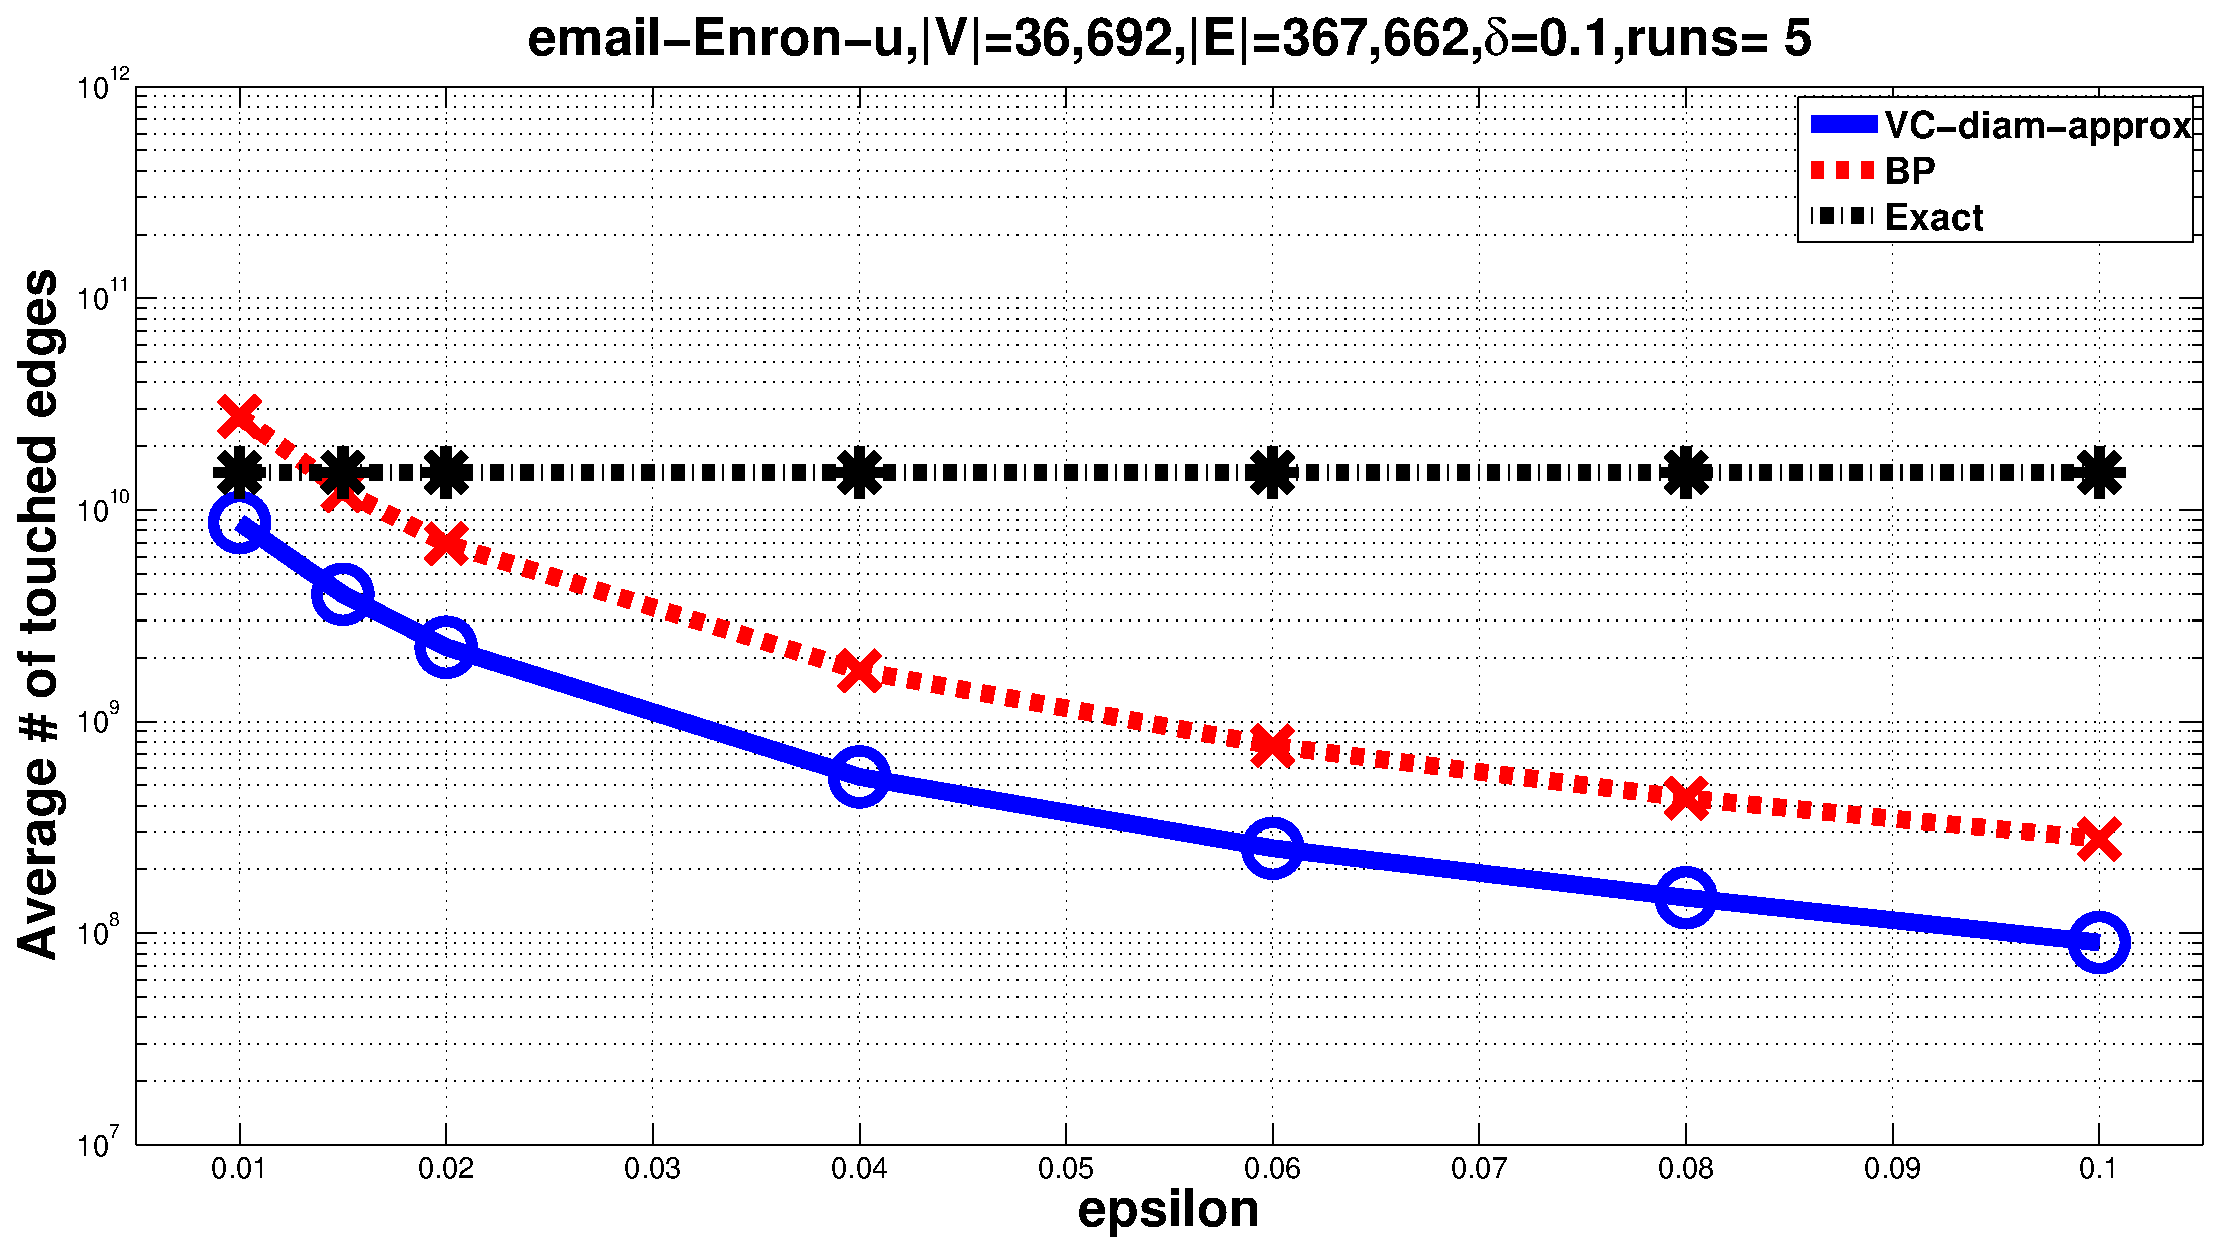
\includegraphics[width=3.8in, keepaspectratio]{email-Enron-edges.eps}
%\caption{Touched edges comparison on email-Enron}\label{fig:email:edges}
%\end{minipage}
\end{figure*}

\subsection{Scalability}\label{sec:scalability}
In Sect.~\ref{sec:discussion} we argued about the reasons why our algorithm is
more scalable than the sampling one offering the same approximation
guarantees~\citep{BrandesP07,GeisbergerSS08,JacobKLPT05}. To evaluate our
argument in practice, we created a number of graphs of increasing size (1,000 to
100,000 vertices) using the Barab\'asi-Albert~\citep{BarabasiA99} and the
algorithms on them, measuring the running time and the number of touched
edges. We report the results in~\cref{fig:random:time,fig:random:edges}. The
theoretically best algorithm would be completely independent from the size
(number of vertices) of the graph, corresponding to a flat (horizontal) line in
the plot. Therefore, the less steep the line, the more independent from the
network size would be the corresponding algorithm. From the figures, we can
appreciate that this is the case for our algorithm, which is much more scalable
and independent from the size of the sample than $\mathsf{BP}$. This is very
important, as today's networks are not only huge, but they also grow rapidly,
and algorithms to mine them need to scale well as the graph sizes increase.

\XXX The figures below are converted from jpg. Need native eps.

\begin{figure*}
  \centering
  \hfill
  \subfloat[Time]{\label{fig:random:time}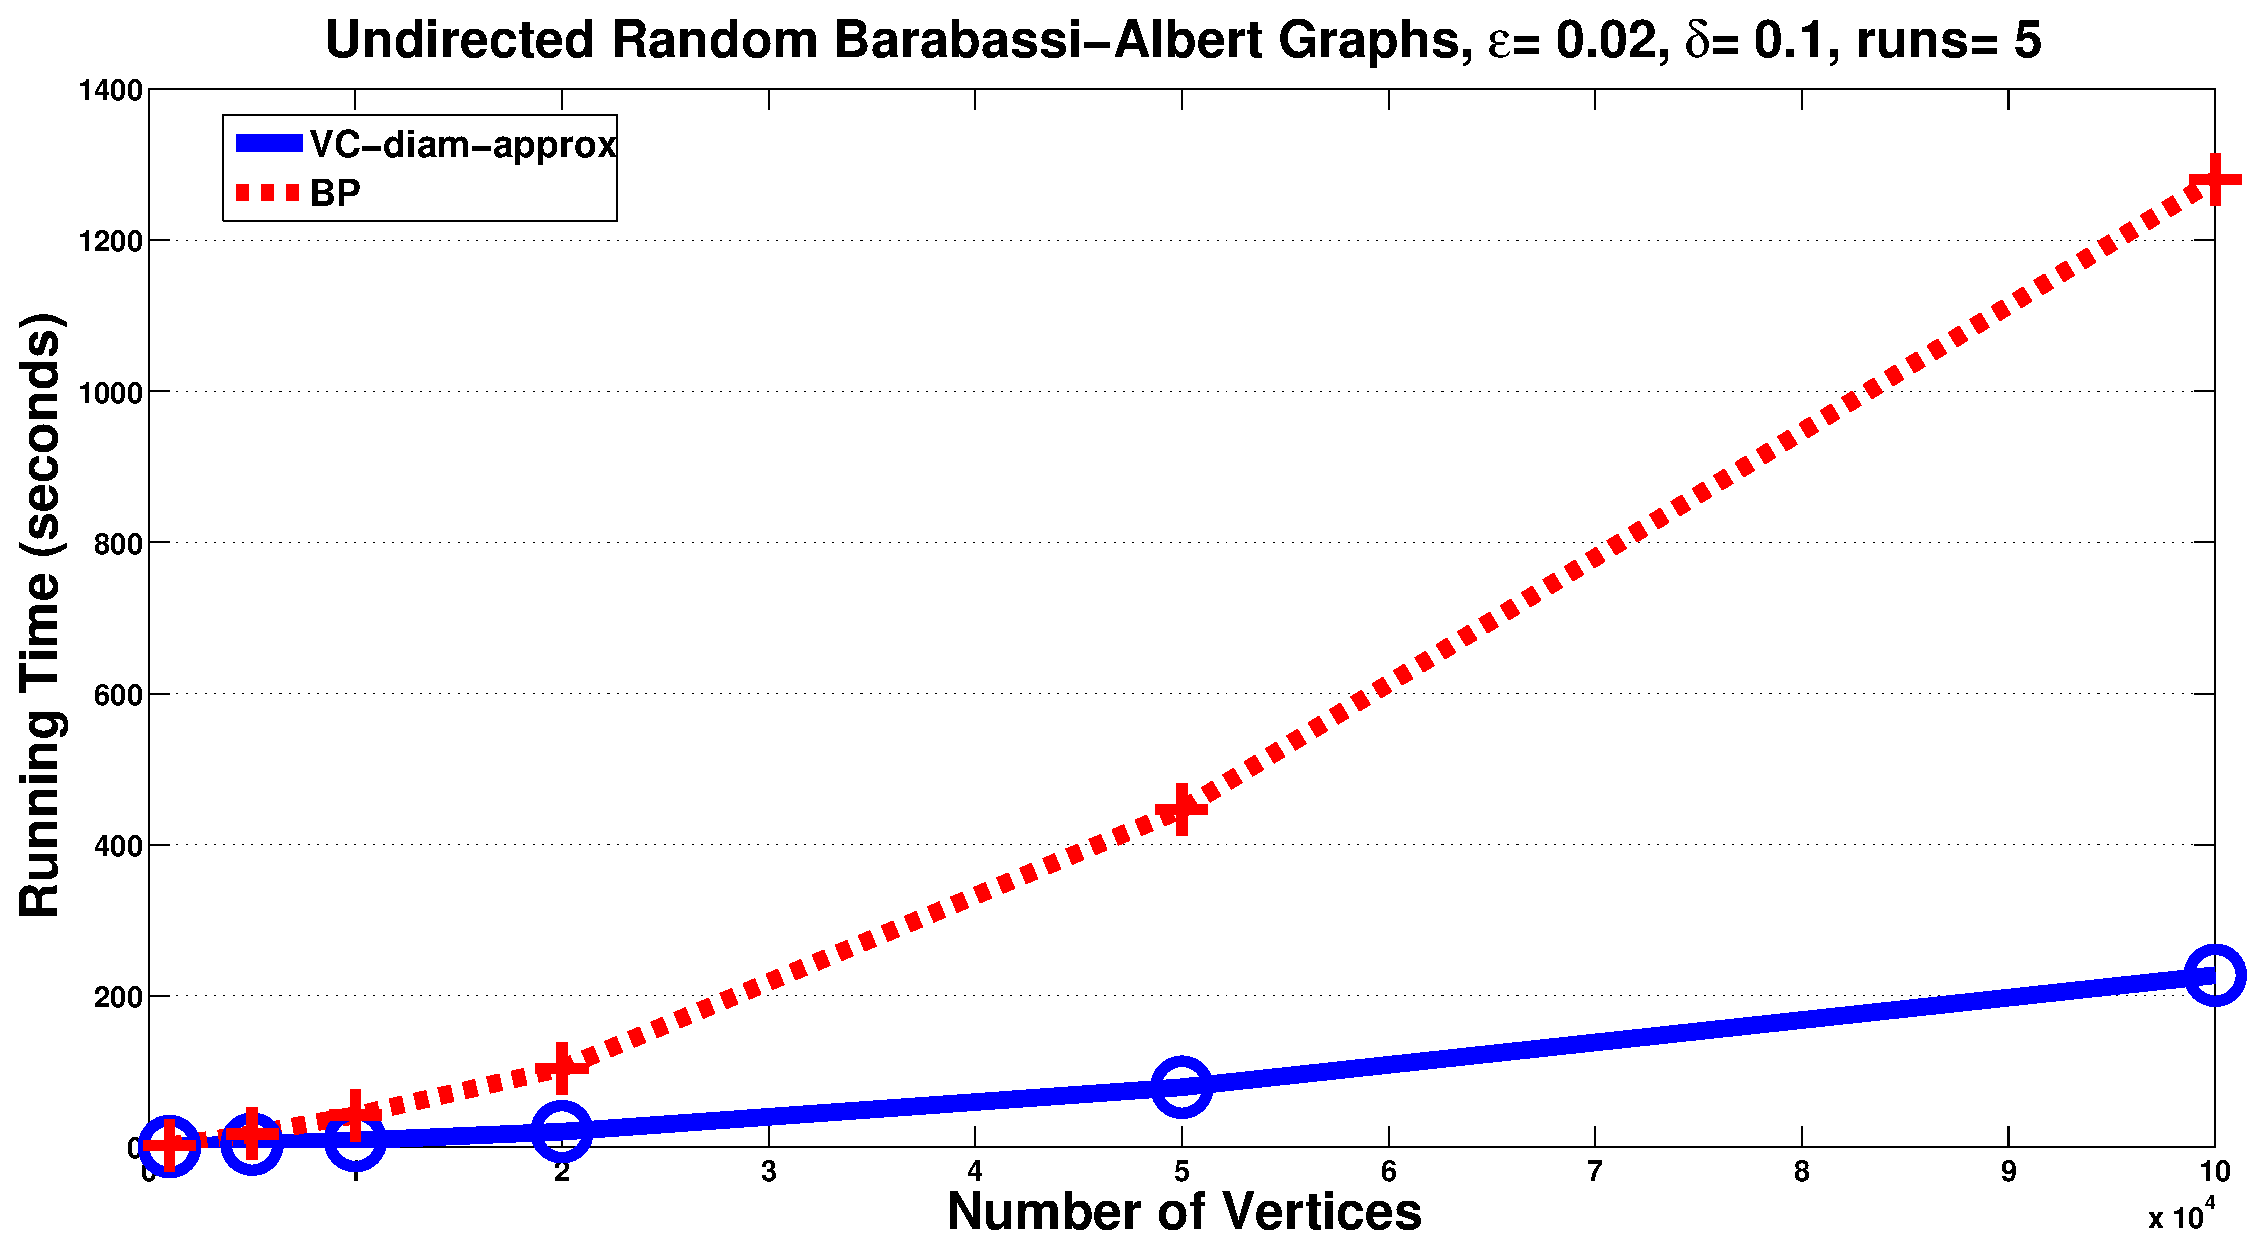
\includegraphics[width=.45\textwidth,keepaspectratio]{random-time}}
  \hfill
  \subfloat[Edges]{\label{fig:random:edges}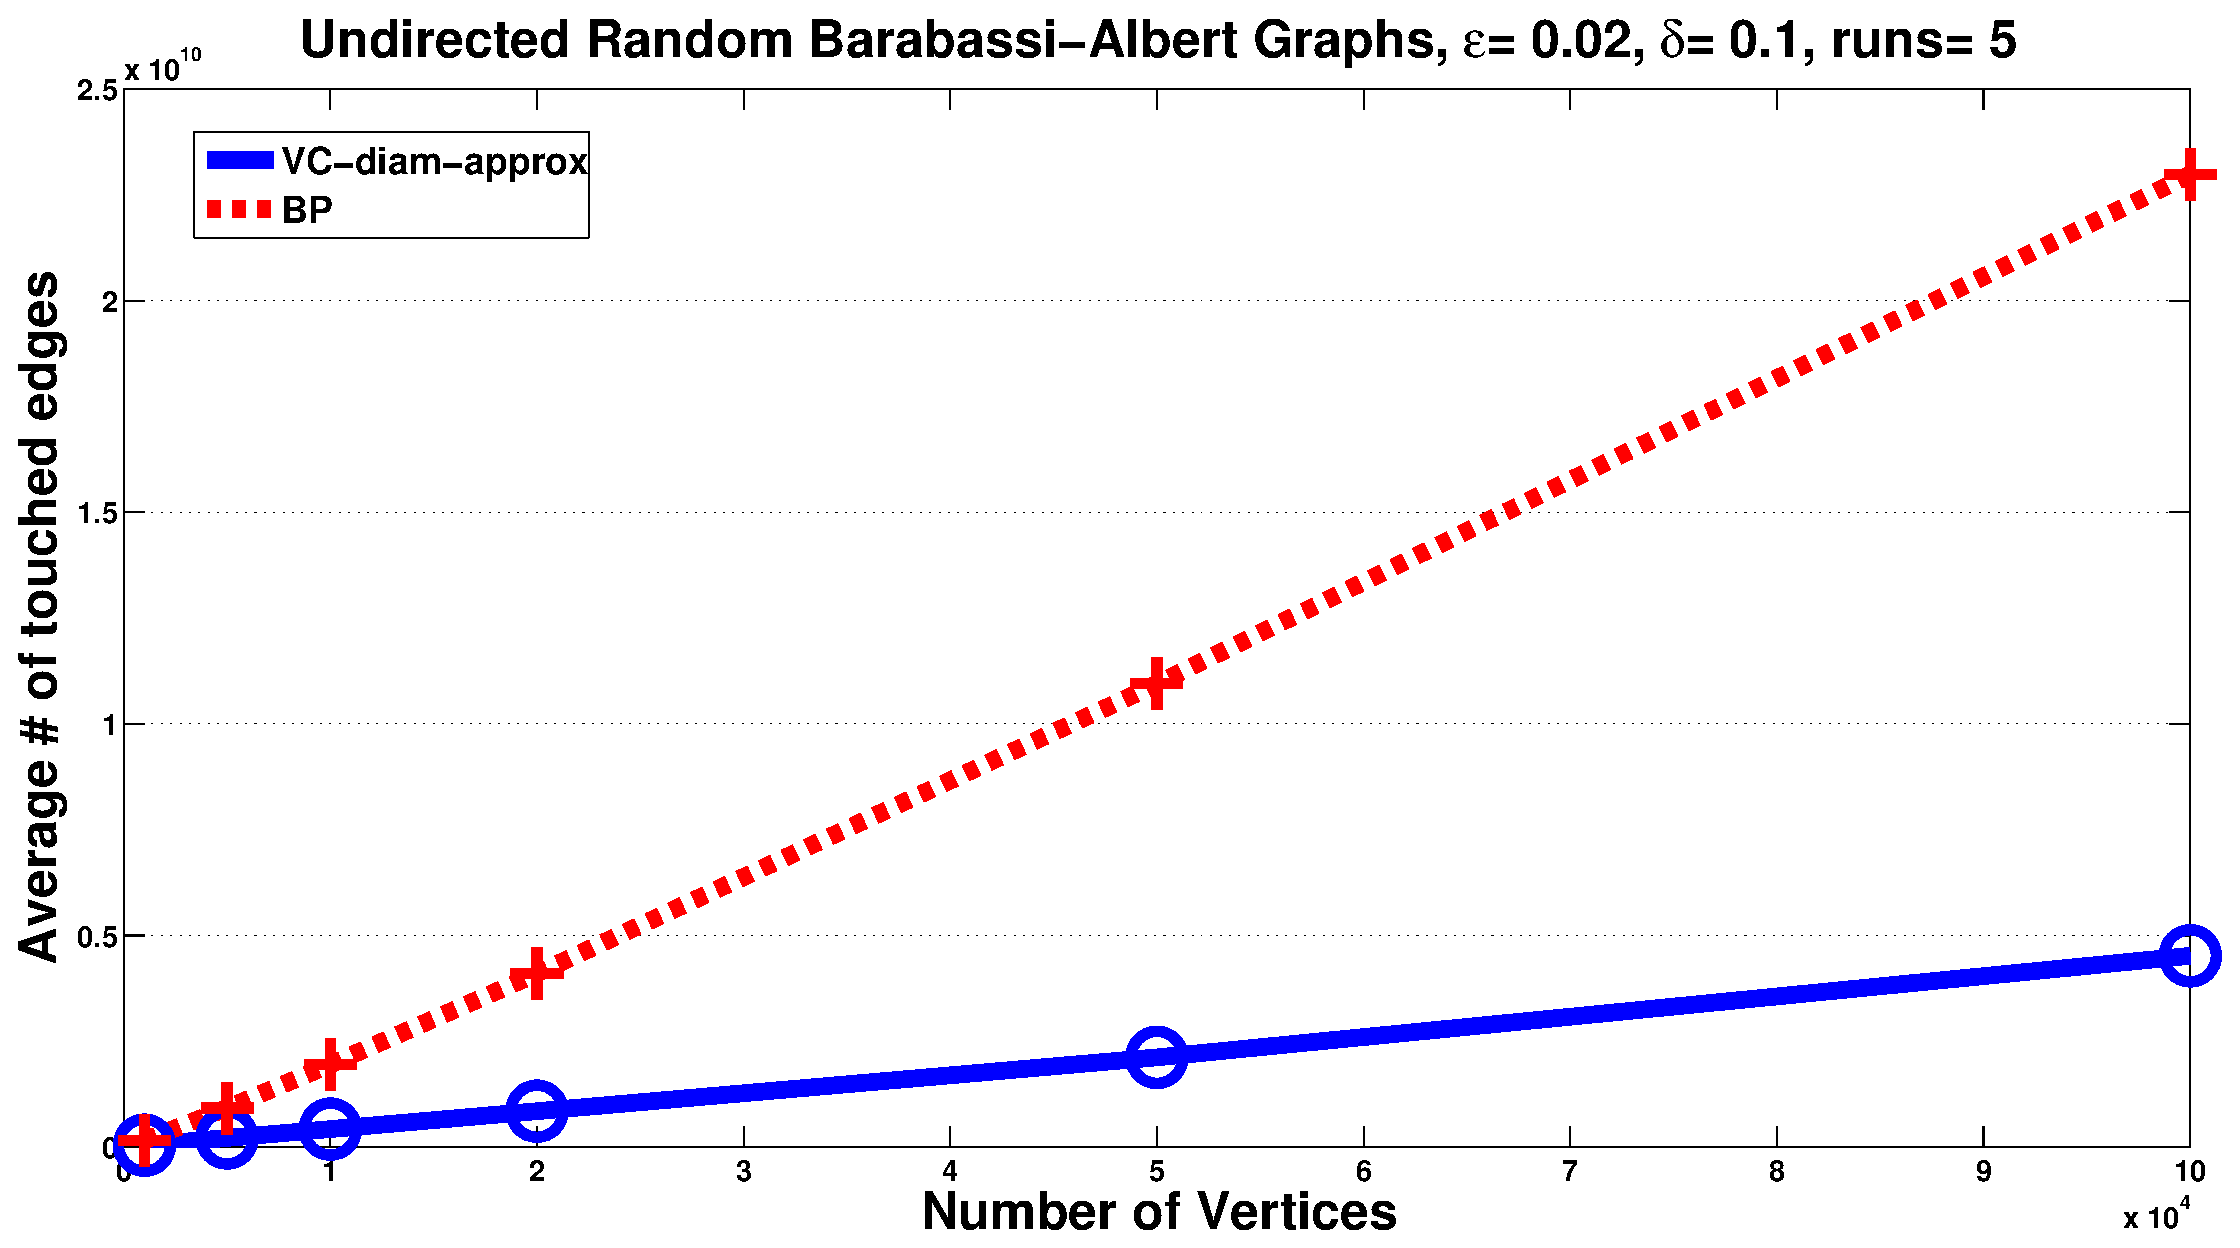
\includegraphics[width=.45\textwidth,keepaspectratio]{random-edges}}
  \hfill
  \label{fig:random}
  \caption{Scalability comparison on random~\citep{BarabasiA99} graphs}
%\begin{minipage}[b]{0.5\linewidth}
%\flushleft
%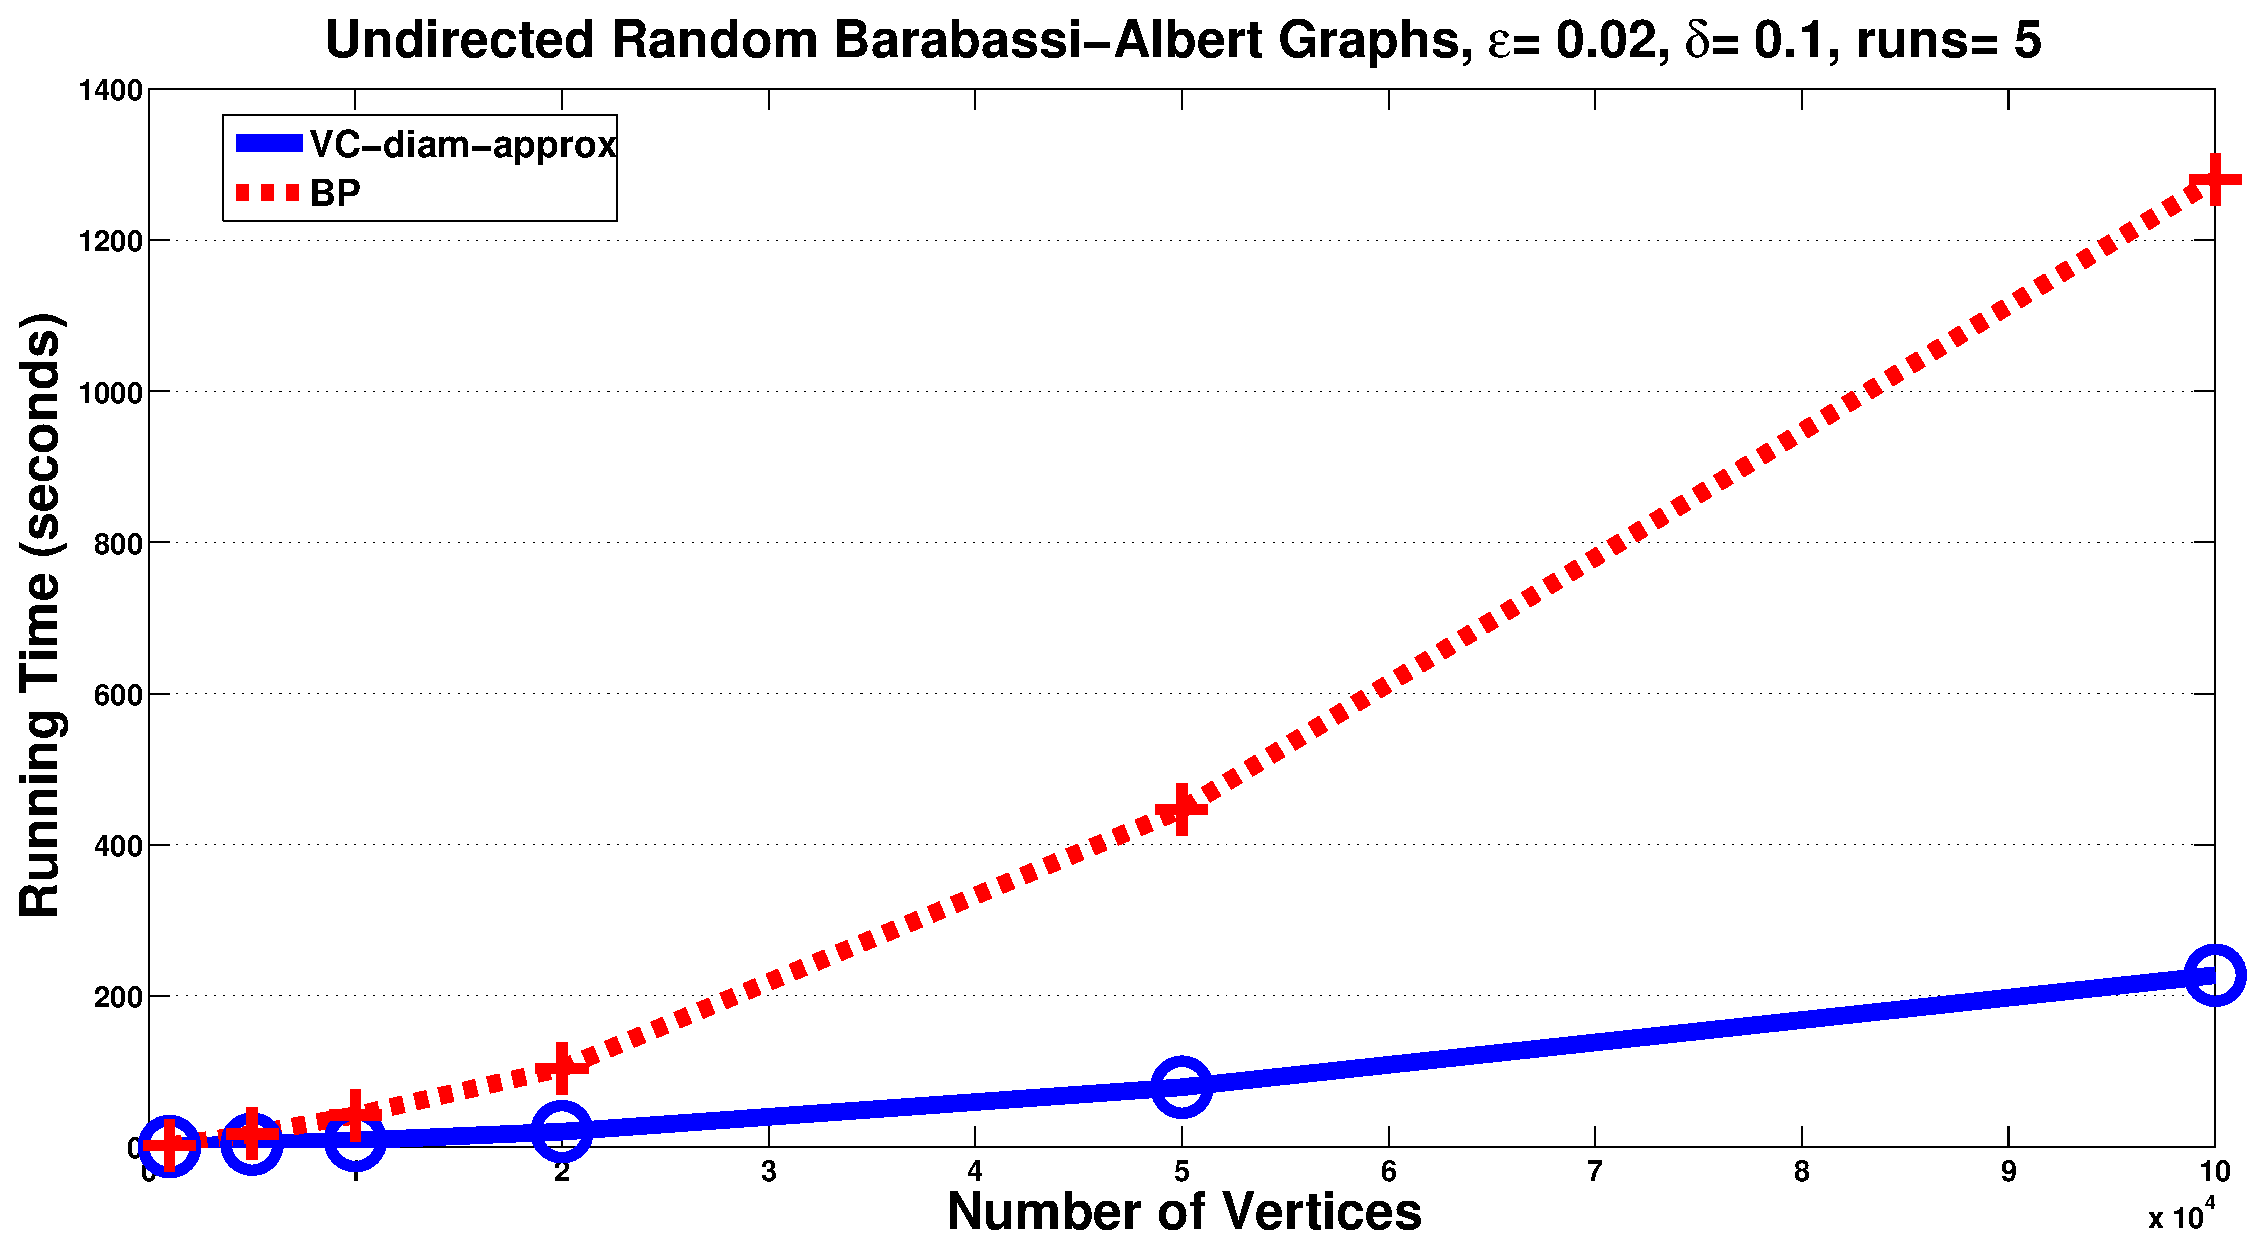
\includegraphics[width=3.8in, keepaspectratio]{random-time.eps}
%\caption{Scalability on random~\citep{BarabasiA99} graphs (time)}
%\label{fig:random:time}
%\end{minipage}%
%\begin{minipage}[b]{0.5\linewidth}
%\centering
%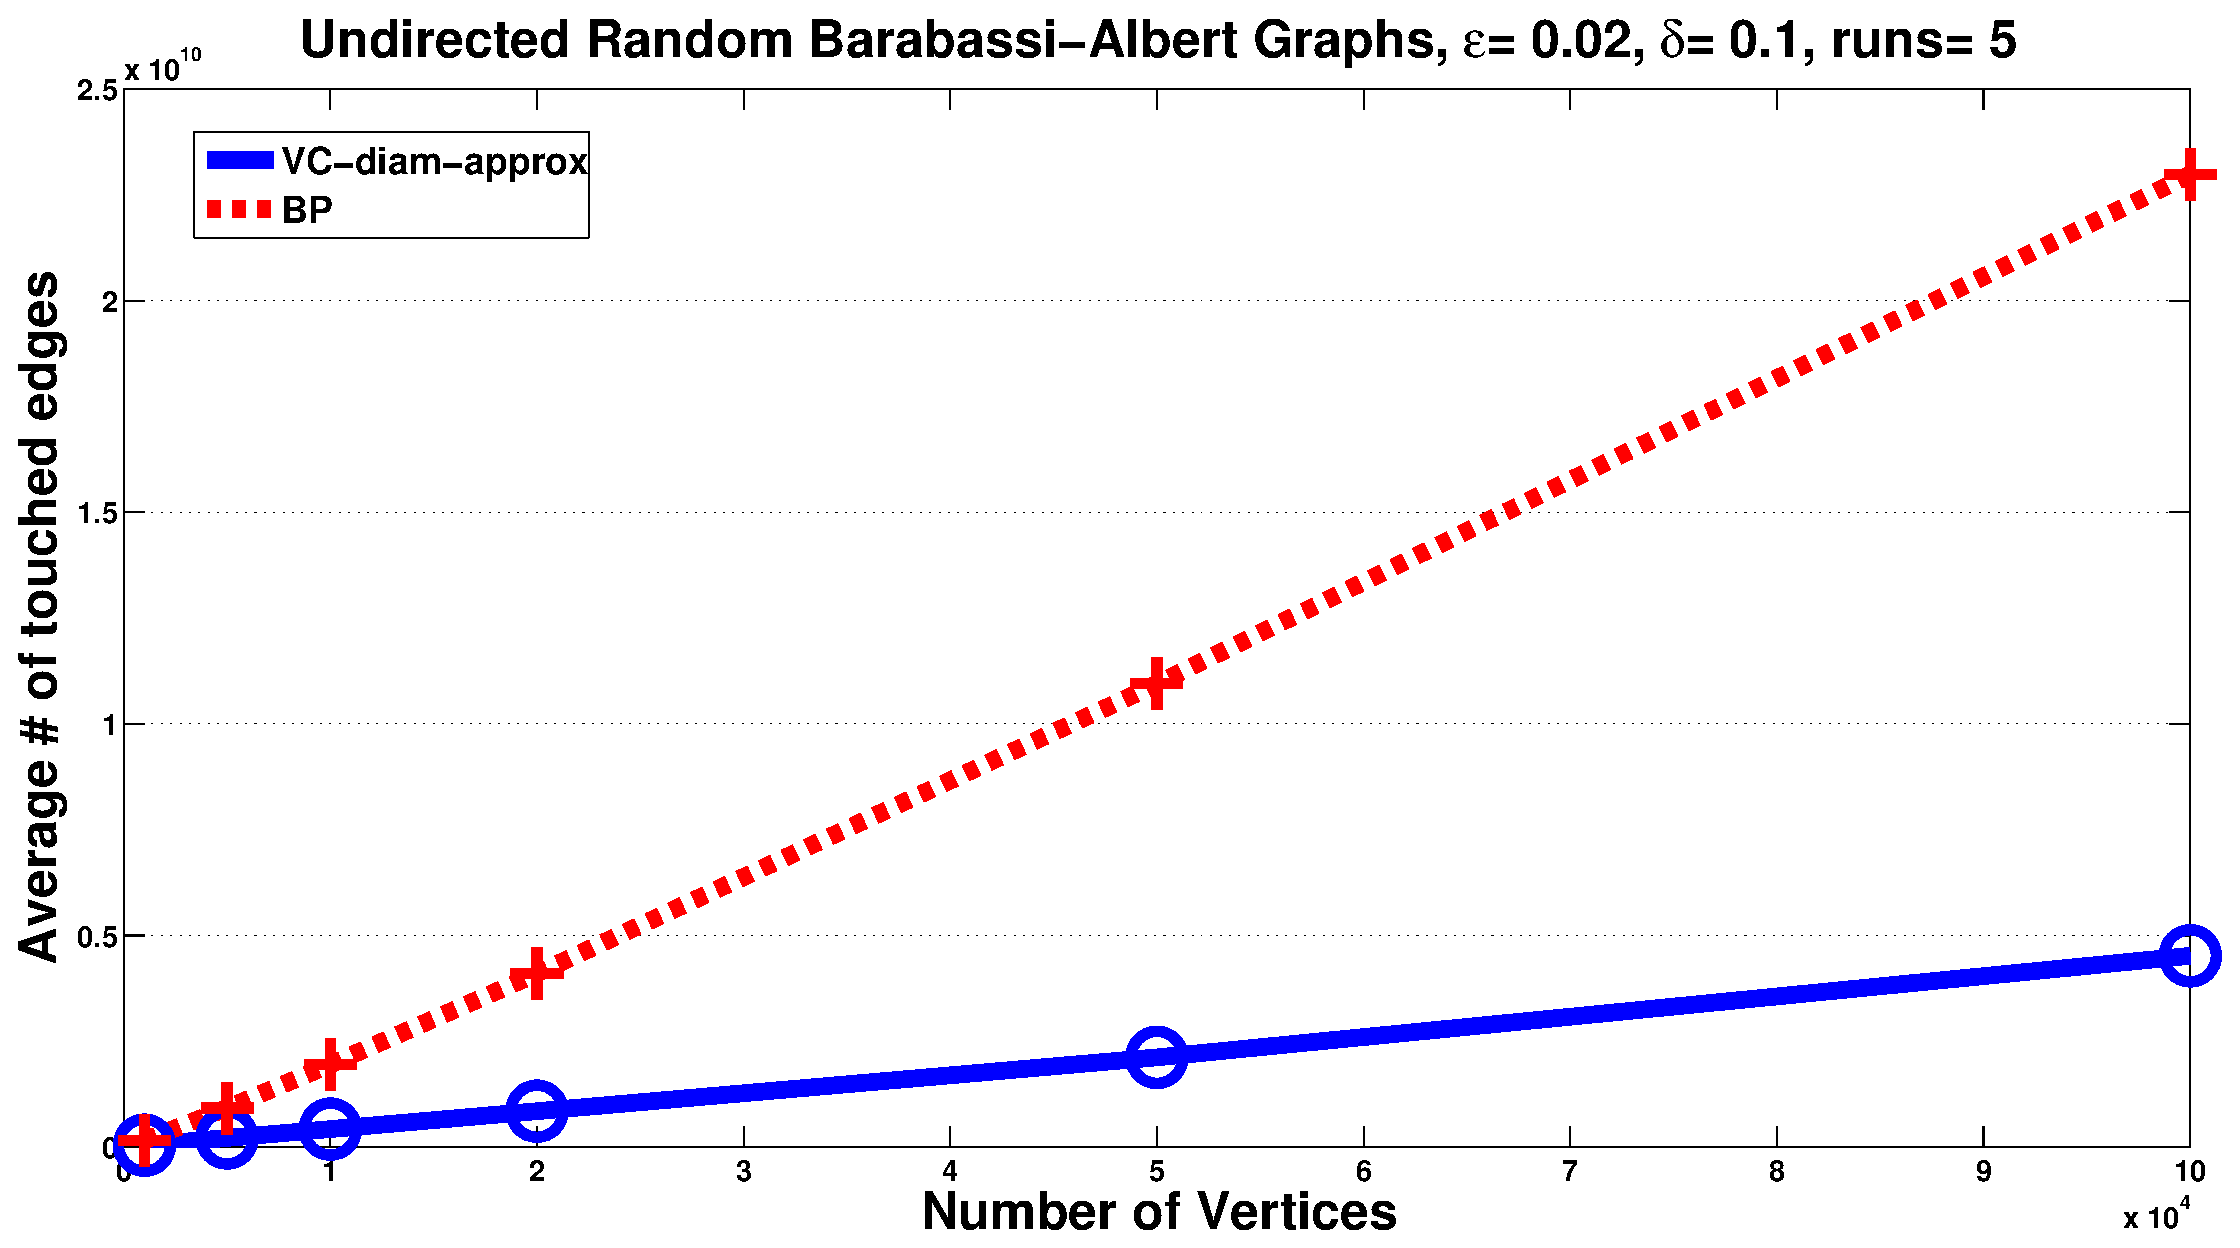
\includegraphics[width=3.8in, keepaspectratio]{random-edges.eps}
%\caption{Scalability on random~\citep{BarabasiA99} graphs (touched edges)}
%\label{fig:random:edges}
%\end{minipage}
\end{figure*}

